\documentclass{pasa}%

\usepackage{graphicx}
\usepackage{float}
\usepackage{booktabs}
\title{Mechanism Lumping - the future approach}
%
%%% Please note that the command \and is not supported in \author.
%\author[Author1]{Author1$^1$, Author2$^2$, Author3$^2$ and Author4$^{2,}$\thanks{This is an example of author footnote}
%\affil{$^1$This is  an example of Affiliation r Author 1}%
%\affil{$^2$This is  an example of Affiliation for Author 2}
%}%
%
%
%\jid{Thesis}
%\doi{10.1019/pas.\the\year.xxx}
%\jyear{\the\year}

\usepackage{aas_macros}
\usepackage{subcaption}
\usepackage{hyperref} 
\hypersetup{colorlinks,citecolor=blue,linkcolor=blue,urlcolor=blue}

%%%%%%% IMPORTANT: We disable hyperlinks by default with this line, to avoid the error "\pdfendlink ended up in different nesting level" while writing.
\hypersetup{draft}
%%%%%%% You may comment or delete the line above to make hyperlinks in your paper active. If you then encounter a strange "\pdfendlink ended up in different nesting level than \pdfstartlink", don't worry! Uncomment the line again, and see https://www.overleaf.com/help/246 for further information.

\begin{document}
%
%\begin{frontmatter}
%\maketitle
%
%\begin{abstract}
%Something here 
%\end{abstract}
%
%\begin{keywords}
%Master Chemical Mechanism - Mechanism - Reduction - Graph Neural Network
%\end{keywords}
%\end{frontmatter}
\onecolumn
\linespread{1.5}

\section{quote}

Abstract thesis: 

As with all scientific xxxxx we are faced with three hurdles. These are Understanding, Improvement and Simplification. Visualiation has long been used for the conveying of important information in our culture. Our brains aare predespositions to absorb images and patterns with far greater efficiency than numbers or characters. We utilise this property to unlock previously unused cognitive capabilities in the understanding of large and complex data. 
Next we consider situations where data is too difficult visualise and apply a series of numerical techneques and metrics to determine what is important and what we might need to measure. 
Finally we look at combining our previously gained knowledge in the simplification and ... of mechanisns... 

\section{INTRODUCTION }


\label{sec:intro}
 
 As science advances, so does our capability to better represent real-world phenomena in the form of simulation and models. This allows for both predictive and evaluative properties for both policymaking, efficiency improvement and climate [refrefref!]. However much of this often comes at a cost. In being able to model, more, and more complex reactions we are often faced with a need for greater computational resources and cognitive ability in the interpretation of the results. \\
 
 
 
 As mechanisms have evolved from having only a hand full of measured reactions, to multiple reactions from a specific protocol, we see an exponential increase in their size (e.g. the addition of isoprene in version 3.3.1 of the Master Chemical Mechanism [MCM] increased it by XX\% compared to version 2). As we near the end of manual mechanism construction, we enter an age where the we can easily generate mechanisms containing the oxidation and degragation processes of new species. Automatic generation software, although overcoming the problem of manual construction and development, often results in mechanisms containing millions of species and billions of reactions. \\
 
 
 
In general there are three main issues that may occur due to a mechanisms size. The simplest of these is the interpretation of the results. As human beings with limited screen real estate and cognitive abilities, we are only able to view or observe a handful of reactions at any one time. With chemistry following a power-law distribution (CITE ChaMBRIDGE) (think 6 degrees of separation), the web of influence is vast, complex and heavily intertwined. This makes the understanding of how each species in a several thousand species simulation change difficult at the least. \\



Next we have the memory requirements required by the integrator. Continuously fetching data from hard storage has a highly detrimental effect on a program. Ideally all components required may be stored on the random access memory during the simulation. As a means to evolve the chemistry, the mechanism (a series of first order differentiable equations) is first integrated and gradded? to produce a relationship matrix of partials - the jacobian. This is an $n \times n$ matrix containing the influence of each species on each other. This means that as our species number increase, the matrix containing these scales by the order of  $O(n^2)$. Since each species does not often contain reactions with many (in proportion to all the other species), a sparse matrix may often be used to circumvent this problem during model execution. However this still poses an issue in both the compilation and preprocessing of these mechanisms, with preprocessors such as KPP[ref] needing to allocate and populate the entire Jacobian matrix, before they are able to create a sparse one for computation. \\


Finally although the mechanism is converted into one set of reactions for integration, this is comprised of many different parts relating to each reaction a species is in. As species rely on many others, this forms a numerically stiff system which cannot be easily, or effectively, parallelised. The computation of all reaction rates for each update of the integrator can prove crippling for the computation time of 3D Earth Simulation Models which can contain complex fluid dynamic simulations and transport between grid boxes. This is seen when comparing the full Master Chemical Mechanism (3.3.1) [RFEF] - a benchmark near-explicit representation of our chemical understanding, with GEOS (Goddard Earth Observing System) -Chem  standard mechanism [REF]: 5809 species, 17224 reactions against 241 species and 719 reactions respectively. 
 
 

\section{Reduction as a solution.}

As mechanisms complexity has long been a problem, many methods of simplification and `reduction' have been developed over the years. Although these are indeed useful, many reduced mechanism often require manual intervention and are usage/case specific. A generalisation of mechanism reduction is the elimination of species and reactions to produce a a smaller, more concise \footnote{and thus manageable}, mechanism whist retaining important properties or features of interest. There are many methods in the literature, the most common of which, are defined below. \\


%The methods of Jacobian analysis and
%overall rate sensitivity analysis proved to be efficient and capable of removing the majority of redundant reactions and
%species in the scheme across a wide range of conditions relevant to the polluted troposphere.\\
%
%The use of the
%quasi-steady state approximation (QSSA) proved to be an extremely successful method of removing the fast time-scales
%within the system, as demonstrated by a local perturbation
%analysis at each stage of reduction. QSSA species were automatically selected via the calculation of instantaneous QSSA
%
%whitehouse pt 1 
%



\subsection{Reaction Removal}
The simplest method of reducing the number of items computed in a model, is to reduce the number of reactions. This eliviates the computational burden of calculating the rate of reaction each timestep.
Classically this was done through the use of Rate and Production analaysis [ref previous chapter]. This allows for the visualisation of each reactions contribution to the rate of change of concentration of a a species of interest. In doing this we can may fillter redundant reactions that contribute less than a certain percentage\footnote{Typically $~5\%$} to the formation of our important species. Other more in depth methods include the principle component analysis of the sensetivity (PCAS), where the most important parameters (the principal components) related to a simulation are selected. Here the objective parameters are those of our important species, and and the investigated parameters are the rate coefficients \cite{PCAS}.


\subsection{Species removal}
Next we have species removal as a method to reduce a mechanism. This is useful not only because it reduced the size of the jacobian, but the removing or combining of species inherently reduces or simplifies the reactions within a mechanism. \cite{whitehouse1} states that using jacobian or sensetivity analysis methods proved `capable' and `efficient' in removing most redundant reactions and species from the MCM. Although there are many methods in which this may be done, all of these tend to partition the chemistry within three groups:


\begin{itemize}
    \item \textbf{Important} - reactions or species directly related to the topic / outcome we are interested in
    \item \textbf{Needed} - reactions/species required by the important species, such that they may perform their desired function
    \item \textbf{Redundant} - those we may remove with little or no consequence to the final outcome of the model. 
\end{itemize}



The interconnected, cascade nature of atmospheric chemistry results in the \emph{important} species containing many dependencies. This means that many of these processes are iterative processes, where necessary species are added to the important species list on each itteration. This is then repeated until either a gap in the chemistry is reached, or more likely a mechanism of the desired size is obtained. There are several methods on how to approach this, some of which are outlined below. 

\subsubsection{Trial and Error}
The simplest method is one of trial and error \cite{tur1990} (Method 1). Here all the consuming reactions of a species are removed. If the resulting deviation between the full and the reduced mechanism is small, then the species may be removed. The downsides of this method is that it may be inefficient for large mechanisms, and only works on a per-species level - you cannot remove like groups. 

\subsubsection{Species Removal by Inspection of Rates}
One of the first approaches to removing species was given by Frenklach in \cite{frenk} with respect to combustion modelling. Here species whose reactions are much slower than the rate determining steps of a mechanism are marked as redundant and removed. 

\subsubsection{Jacobian Connectivity Method}

The log-normalised Jacobian matrix can be used to determine the change in production of a species due to a 1\% change in the concentration of any other species. In squaring the effect of this for all improtant species, we get a metric depicting how the change in a certain species affects the concentrations on all important species, \autoref{connectivity}, where $({y_i}/{f_i})({\partial f_i}/{\partial y_i})$ is element $i$ of the normalised Jacobian . Through an iterative process we can identify redundant species, of a low contribution to our important species, and remove them. This is known as the Connectivity Method \cite{cm}.


\begin{equation}
B_i  = \sum_j(({y_i}/{f_i})({\partial f_i}/{\partial y_i}))^2 \label{connectivity}
\end{equation}

\subsection{Lumping}
Rather than removing species or reactions from a mechanism we may combine them to form a new composite species. This is species lumping. To do this we must first consider how we determine species that are to be joined together, and then how their grouped reactions will contribute to every other species it reacts with. Some of the more general types of lumping styles are outlined below. 


\subsubsection{Chemical Lumping}
Mechanisms follow protocols in their generation. This produces reaction styles that many like-structured species follow in their degregation. In determining such classes we may be able to generalise like-species reactions and group them together as one. Taking the CRI mechanism as an example, this has taken the Ozone production capability as a feature of interest. The rato of CC and CH bonds are used to determine a species oxidation possibility ... An example of this are species such as CARB9  ... some examples and what the names mean \\

As this type of lumping has already been performed on our starting mechanism, we shall not be applying it any further. 


\subsubsection{Linear}
\subsubsection{Lifetime}
\subsubsection{Quasi Steady State Approximation (QSSA)}
QSSA works on the axiom that the the flux through a species is 0  - Use louise whitehouses thesis here (better description that the analysis to kinetic reactions book)

\subsection{Graph parallels. }
Although there are many graph based methods that exist within the reduction realm, most of these concentrate on the generation of skeletal methods through the building of a directed tree (subcategory of graphs from source to target) - LIST of refs and sentence of all skeletal methods. Path flux analysis (Sun et al 2010)\\

Instead we may find ourselves applying graph theory to solve other reduction methods. For instance we can trace back influence through connecting edges using dijkstras shortest path algorithm (CH2 ref) - analogous to the connectivity method, or a leave one out approach combined with pagerank to access the effects of removing a node.\\

We can use the graph structure to analyse changes of reactions or relationships between species. This can provide an alternative representation and method to access such data. Additionally we may use graph clustering techniques to locate groups of highly connected, fast reacting/strongly related species. This has applications in both understanding the data, but more importantly chemical lumping. In creating a graph from the mechanism, we not only encode information about the chemical structure, but also the rate of reaction in the graph. In grouping species by high numbers of reactions between them with fast fluxes we can take a QSSA style approach to reduction, and assume that since the rate of reaction between them is much much faster than those outside a cluster, they may be grouped together. This will be explored in PART II [ref link].



\section{Methodology: Part I }
In this chapter we are not interested in reducing a mechanism for a certain case study or environment. Instead we look at tools capable of simplifying the hard coded maths behind the reactions that exist within the atmosphere. Since the key chemical drivers differ from location to location we make use of our ability to run a range of different simulations which provide an overview of the entirety of the input space (intial concentrations). Although this may not replicate and real-word (physical) scenarios, it tests the robustness of the mathematics behind the mechanism and in using this data to predict like properties based on the physical equations which describe the system. We work on the assumption that these have been correctly fitted and tested against experimental data, and that through reducing the mechanism based purely on its mathematical response to different conditions, its ability to predict atmospheric science will be preserved. \\

The model setup shall be defined below. 

\subsection{The Mechanism}
The mechanism we wish to use as a baseline is the Common Representative Intermediates (CRI) Mechanism of version 2.265 ,\cite{criv2}. This is an update to the CRI v2.0, with the purpose of updating the chemistry to better represent that of MCM version 3.3.1 (i.e. the inclusion of explicit Isoprene chemistry). The CRI v2.265 mechanism has been developed much in the same way as its precursor, and is centred around describing the ozone formation from Volatile organic compounds (VOCs) in the troposphere. The main assumption behind the lumping in the generation of this mechanism is that `the potential for ozone formation from a given volatile organic compound (VOC) is related to the number of reactive (i.e., CC and CH) bonds it contains',\cite{cri}. Reductions are made on a compound-by-compound basis and compared to the MCM using a series of 5 day box-model simulations. \\

The CRI v2.265 mechanism contains 422 species and 1261 reactions. This is still almost double of those within the global GEOS-Chem model. With explicit manual reduction being used to reduce the MCM by YY percent, we wish to apply a series of automated reduction techniques and compare them to the baseline mechanism. We chose the 2.265 version of CRI, since it posesses both a potential for further reduction (CRI v2.0 was reduced a further 5 times); there are a sufficient number of items to make it a non-trivial example, but mainly as its relative size is just within our ability to visually inspect the output of each species. 

\subsection{The Box-Model}
The box model used shall be an adapted version of the Dynamically Simple Model of Atmospheric Chemical Complexity (DSMACC) [ref doi, ref DSMACC]. This has had several changes which allow for multiple parallel runs, easy extraction of rates, fluxes and the jacobian matrix as well as a simple ncurses interface for loading and parsing new files. \\

The DSMACC model works by using the Kinetic Pre Processor (KPP) [REF] to generate Fortran code, which can then be used to integrate the provided mechanism. As there were some issues presented with this a pre-pre parser code was used on the mechanism before running KPP, and a post parser on some of the files to provide the desired output. 

\subsection{Model Inputs}
As we do not wish to constrain results to a specific case example, we provide a range of inputs with the aim of covering all possible concentration combinations. As a means of determining all non-lumped species within the CRI mechanism, we only used those which appear in both the MCM and CRI. This also ensures that should it be desired at a later date, any further reduced mechanisms can directly be compared with the results of the full MCM. \\

In terms of sampling there are several types that may be used ,\cite{sampling}. The main or most common is Random, or Monte Carlo, sampling. The problem with this is that its pseudo random nature may often results in regions of high density and some of low, \autoref{fig:mc}. In attempting to sample the entirety of our input space we use a method based on the principles of a Latin square. A latin square is a square containing n items, arranged in such a way that they only appear once in each row and column, much akin to a sudoku puzzle ,\cite{lsq}. A latin hypercube is a generalisation of this allowing for an alternative subspace sampling to the monte carlo method which expands the probabilistic stratified-style sampling of a latin square into n-dimentional space. This presents better covarage of our input space \autoref{fig:lh}  and will be used with the following limits, TAABLE, to gen our sample simulations.

\begin{figure}[H]

\begin{subfigure}{.5\textwidth}
  \centering
  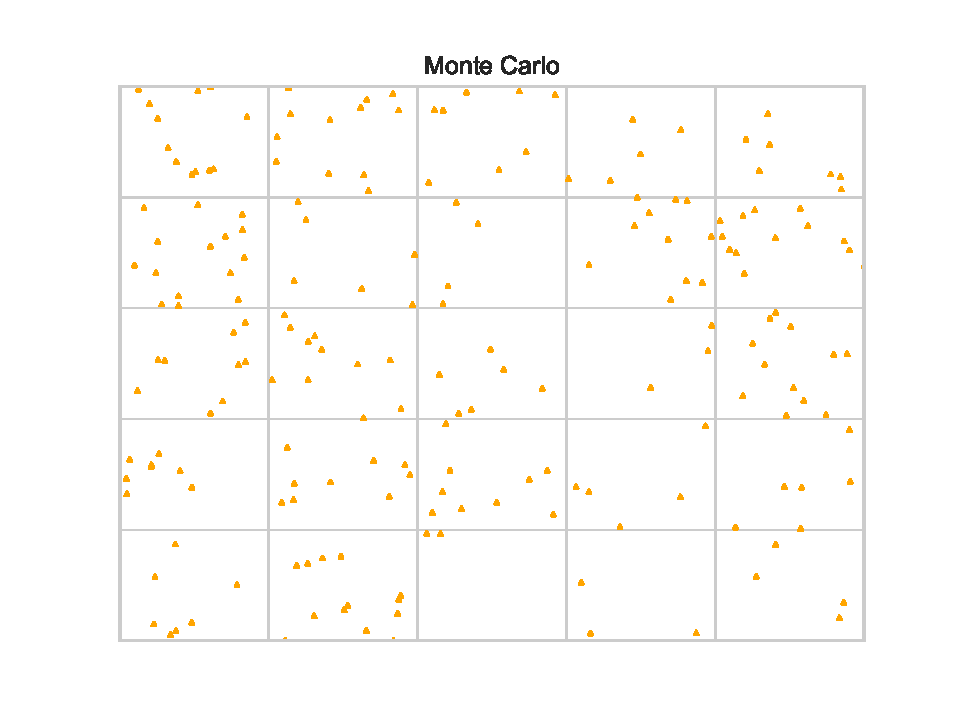
\includegraphics[width=\textwidth]{fig/mc.pdf}
  \label{fig:mc}
\end{subfigure}%
\begin{subfigure}{.5\textwidth}
  \centering
  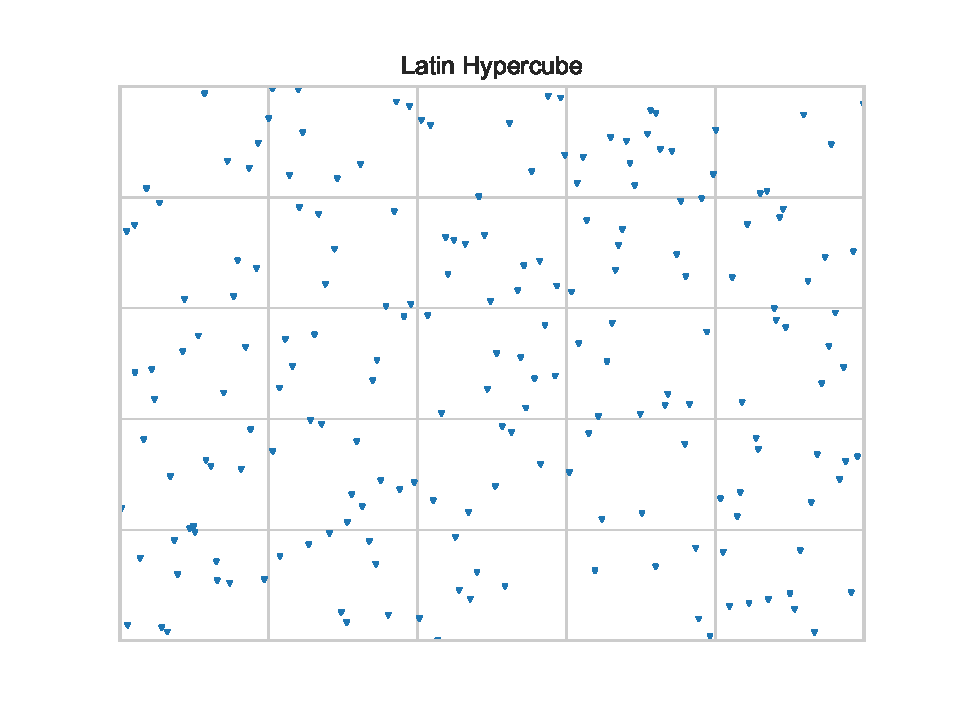
\includegraphics[width=\textwidth]{fig/lh.pdf}
  \label{fig:lh}
\end{subfigure}%

\caption{A comparison of the distribution of 250 sampled points using a) Monte Carlo and b) Latin Hypercube sampling}
\end{figure}


\begin{equation}
\text{concentration}
    \begin{cases}
      min = 10^{-8} \ max=10^{-13} , & \mathbf{if} NO,NO_2,O_3\\
      min = 10^{-8} \ max=10^{-13} , & \text{otherwise}\\
      
    \end{cases}
  \end{equation}

\subsection{Reduction through Lifetime}





\subsubsection{Calculating the lifetime}
Within models a species lifetime is regarded as the time taken for its concentration to halve [ref]. This works on the assumption that the species is not produced, and that rate coefficients and other constants remain constant. For a first order decay of sample \autoref{eqn}, we can represent the decay using \autoref{decay}, showing that the half life is independent of initial concentration. 

\begin{equation}
A \rightarrow{^k} B
\label{eqn}
\end{equation}

\begin{equation}
s(t) = a_0 \exp(-kt) \\
\frac{a(t)}{a_0} = \exp(-kt) \\
$$linearised this gives$$
\ln (\frac{a(t)}{a_0}) = -kt
$$ after $\tau_{1/2}$ the concentration is equal to $a_0/2$ of initial rate $a_0$, which gives $$
\ln(\frac{\frac{a_0}{2}}{a_0}) = \ln(\frac{1}{2}) = \ln(2^{-1}) = -\ln2 = k\tau_{1/2} 
$$$$
\tau_{\frac{1}{2}} = \frac{\ln 2}{k}
\label{decay}
\end{equation}

In species of the first order only, this may simplified to 
\begin{equation}
a(t) = a_0 \exp (t  \sum_j k_j )
$$ and therefore the half life may be written as the reciprocal sum of rate coefficients: $$
\tau_A = 1 / \sum_j k_j
\end{equation}

and is how lifetime is calculated for photochemical species [ref! pillin and seakins]. An alternative method for half life calculation may be obtained using the diagonal (self reference) of a Jacobian matrix ,\cite{kinetics}:

\begin{equation}
\tau_1 = - \frac{1}{J_{ii}}
\end{equation} 

This value will usually be negative unless a species does not contain a consuming reaction, then it will be zero. 


The xxxxx method of reduction consists of the isolation of species with similar lifetimes and reactions as a means of lumping. In doing so the ... etc 


\subsection{Comparing Magnitude and Direction}
Since the photolysis reactions in a model change the resultant rates, and thus flux of a species depending on the azimuthal angle related to the time of day, we not only want to compare species with the same magnitude, they also need to match the profile as they change. To do this we may represent all pariwise species matches on a latent space representing the size and angle between their temporal vectors. This is done through using the euclidean distance on the $x$ axis, and cosine distance $y$ on the $y$. 

\subsubsection{Euclidian distance}
This is the simplest method of vector comparison and works by calculating the distance between all points in two vectors. For the vectors

\begin{equation}
v1 = [ a,b,c, \dots n ] 
$$$$
v2 = [ i,j,k, \dots z ]
\end{equation}

This can be done using pythoagoras' theorem in \autoref{euclid}:

\begin{equation}
e_{dist}  = \sqrt{(a-i)^2 + (b-j)^2 + (c-k)^2 + \dots + (n-z)^2}
\label{euclid}
\end{equation}

This transformation converts the straight line distance between each vector into metric space, allowing us to represent the difference in their magnitudes as a single scalar. Unfortunately as this requires the difference between all permutations of rows, it cannot be done as a single operation, but as multiple. \\

APPLICA"tiion

\subsubsection{Cosine Distance} 

Similarly if we wish to calculate the angle between two vectors we may use the cosine difference. In starting with the definition of the dot product 

\begin{equation}
v1 \cdot v2 = \|v1\|\|v2\| \cos \theta
$$this may be arranged$$
\cos \theta = \frac{ v1 \cdot v2}{\|v1\|\|v2\|}
\end{equation}

Since this does not work for the triangle ? inequality, we need to normalise each vector before calculating the cosine distance. The merits of this come from  ... which makes its application comparing the similarity between texts or documents of different sizes very popular (REF!). \\


COMPARE force graph of cosine differences and force graph of euclidean distances. Colour ones close to eachother. \\



\subsection{The Auto-Encoder (AE)}
Auto-encoders are a subclass of neural networks which are primarily used for dimensionality reduction. Rather than predicting a numerical output autoencoders focus on the construction and deconstruction of data through the use of an encoder and decoder pair. The encoder takes an n dimensional input and applies a compression, reducing it to the number of dimensions in the bottleneck layer. This reduced dataset is then reconstructed within the decoder. Such a process not only allows for an easy understanding in the error of the reduced data, but can also be used in the filtration of noisy or pixelated data [ref].\\ 


\begin{figure}[H]
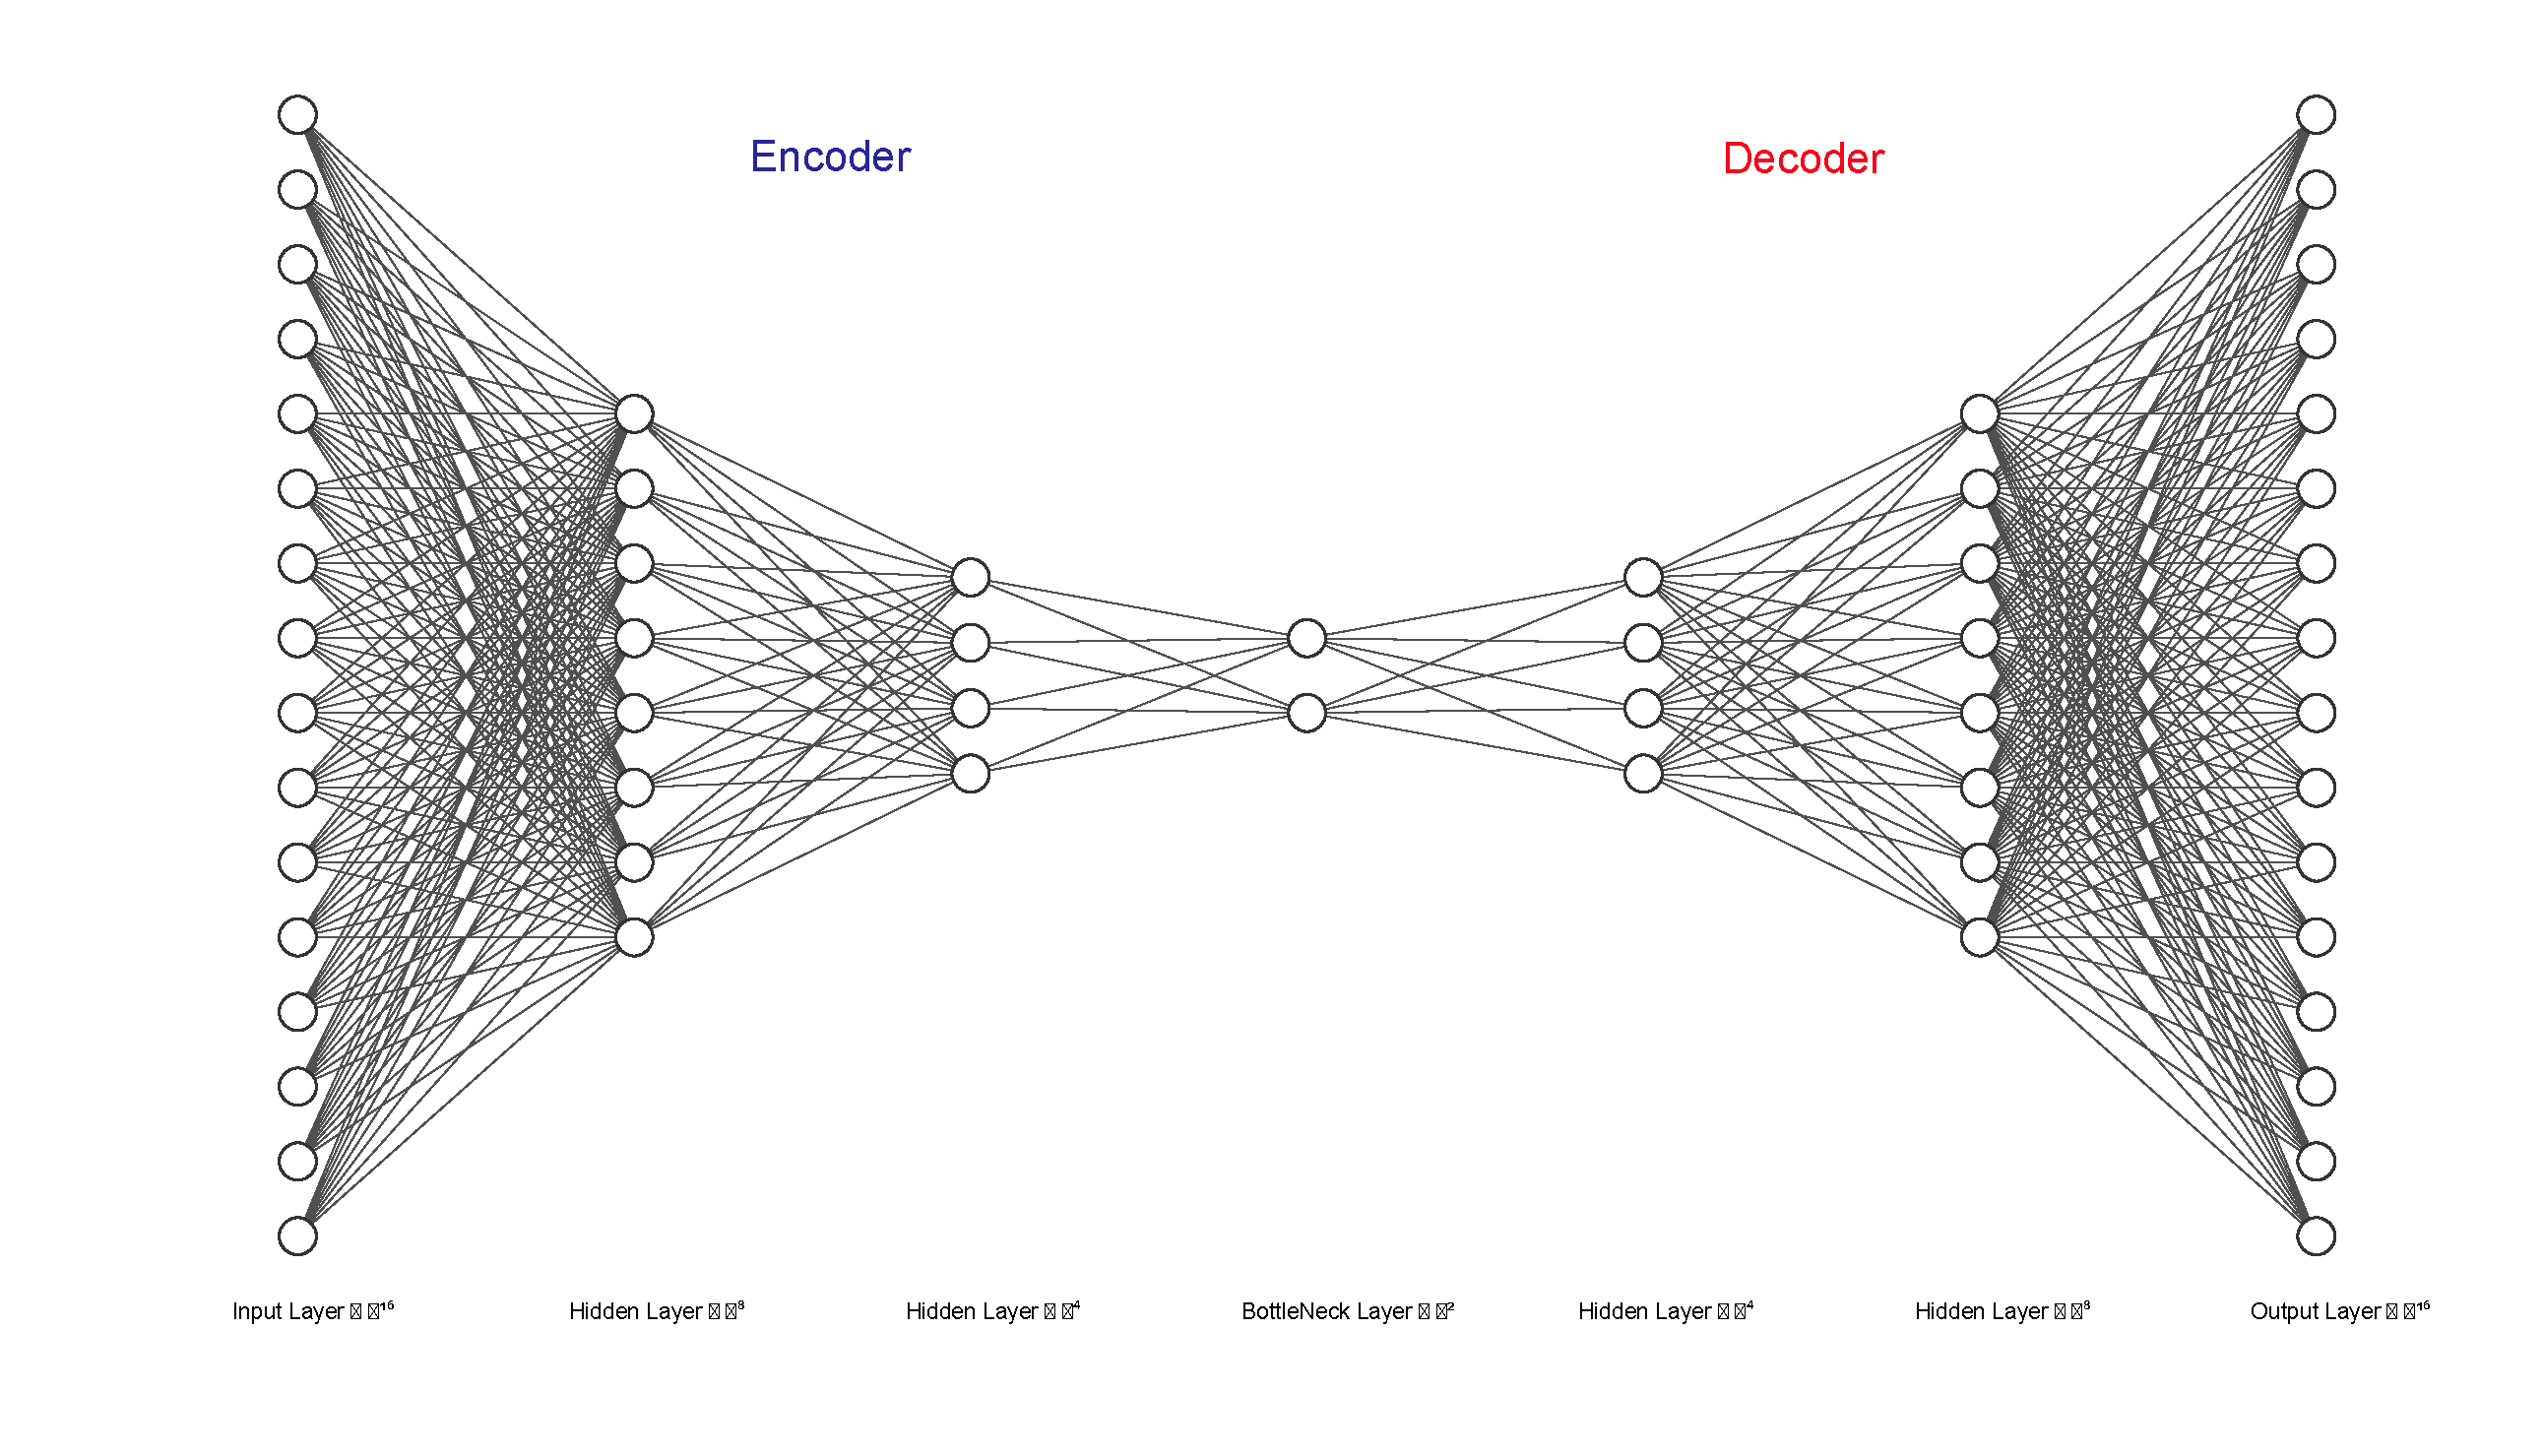
\includegraphics[width=\textwidth]{fig/ae.pdf}
\caption{An example autoencoder structure which reduces a 16 dimentional input to 2. Draw with the aid of \cite{drawae}}
\end{figure}


Usage in image reconstruction, signal processing or feeding large data into other models. \\

There are two features of an autoencoder that make it powerful. The first is the ability to sample your latent space using the decoder. This means we are able to establish features that correspond to gaps between our datapoints - which can have its application if the data used is sparse or incomplete. Next comes the inherent non-linearlity of the model. As an autoencoder is just a neural network, the amount of information passed through each link between layers is governed by an activation function. Should this activation function be linear, the reduced dimension will be much akin to a PCA decomposition. However unlike PCA, in reducing the number of dimensions, we do not discard any data, but rather combine it - as per the nature of the links of the network. In trying to model/fit non-linearity, we have a range of activation functions to choose from. These are:

\subsubsection{Activation Functions}

\paragraph{Binary Step}.\\\\
This is a simple threshold function. If the input is above the threshold, the message is passed on. This makes it efficient, but unable to classify a single input into multiple categories. This can be likened to a yes|no decision tree. 

\begin{equation}
f(x) = 
    \begin{cases}
      1 , & \mathbf{if} \ x < threshold \\
      0 , & \text{otherwise}\\
      
    \end{cases}
  \end{equation}

\begin{figure}[H]
\centering
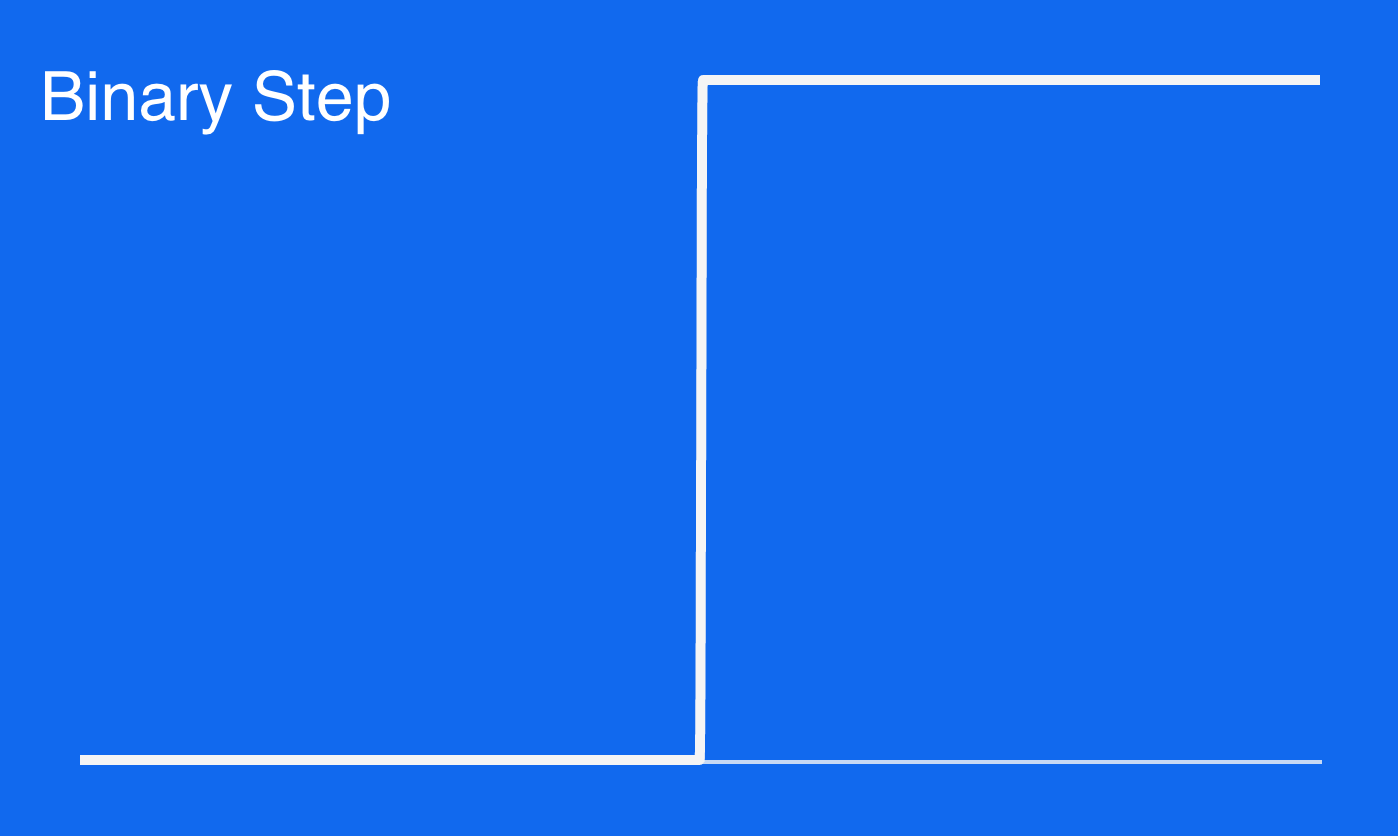
\includegraphics[width=.265\textwidth]{fig/binary.png}
\caption{Binary Step activation function.}
\end{figure}



\paragraph{Linear}.\\\\

This produces a signal proportional to the input multiplied by each neurons weight. It is an improvement over the step function as it allows for multiple outputs. It does however mean that we are unable to use backpropagation (gradient descent) to train the model. In adition to not being able to improve a model, all the layers in the neural network collapse into a single layer. This means that the final layer will always be a linear function of the first layer. This eliminates all the merits which may be gained from deep learning. A neural network with a linear activation function is simply a linear regression model. 

\begin{equation}
    f(x) = m(x)
\end{equation}
\begin{figure}[H]
\centering
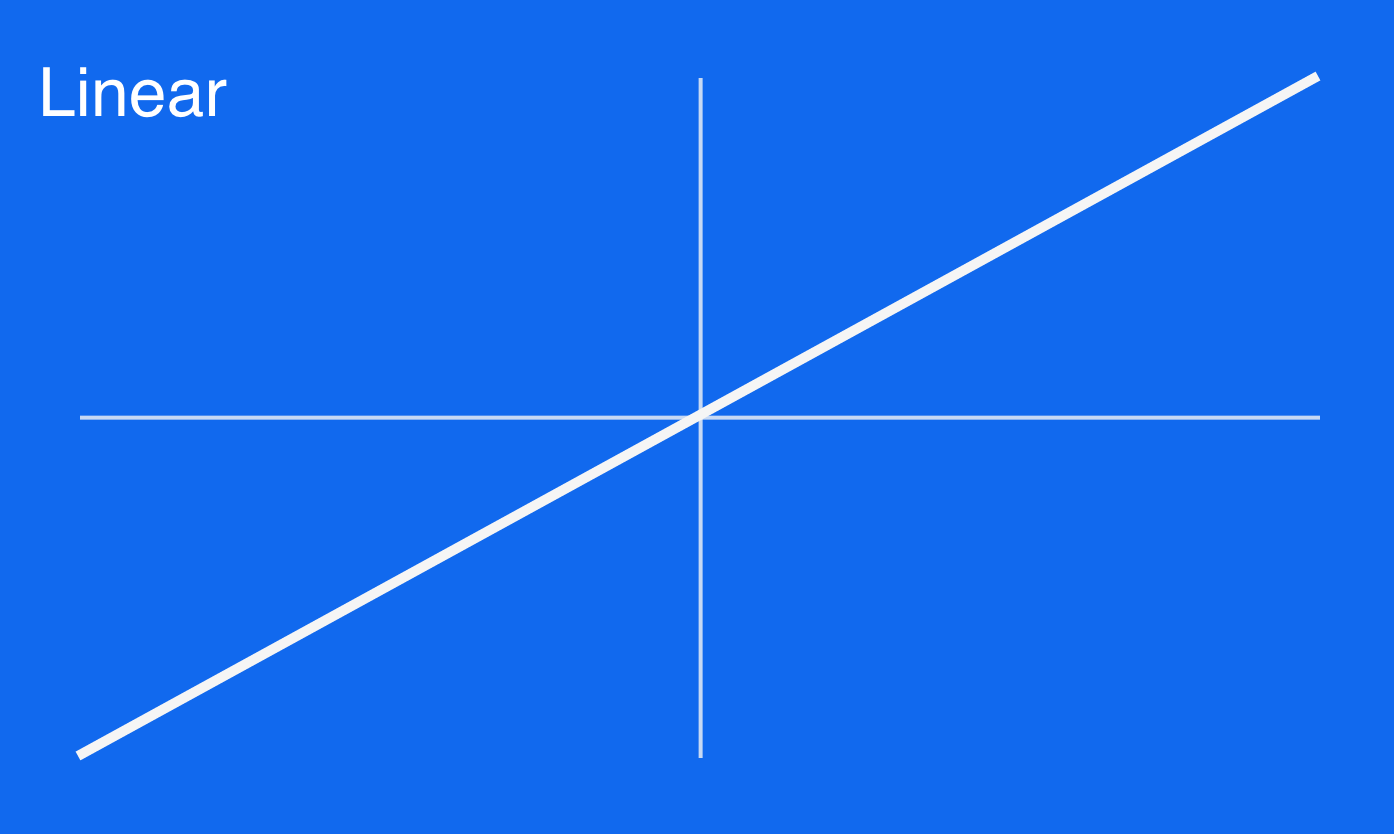
\includegraphics[width=.265\textwidth]{fig/linear.png}
\caption{Linear activation function.}
\end{figure}

\paragraph{Sigmoid / Logistic}.\\\\
The first of the non-linear activation functions. It has a smooth gradient providing smooth output values which are bound between 1 and 0, normalising the output of each neuron. The main disadvantage is that is falls foul the vanishing gradient problem - for extreme values of $x$ there is close to no change in the prediction. This may result in either early termination of the training, or a slow training cycle in obtaining adequate precision. The activations is computationally expensive and the outputs are not zero centred. 

\begin{equation}
    f(x) = 1/1+e^x
\end{equation}
\begin{figure}[H]
\centering
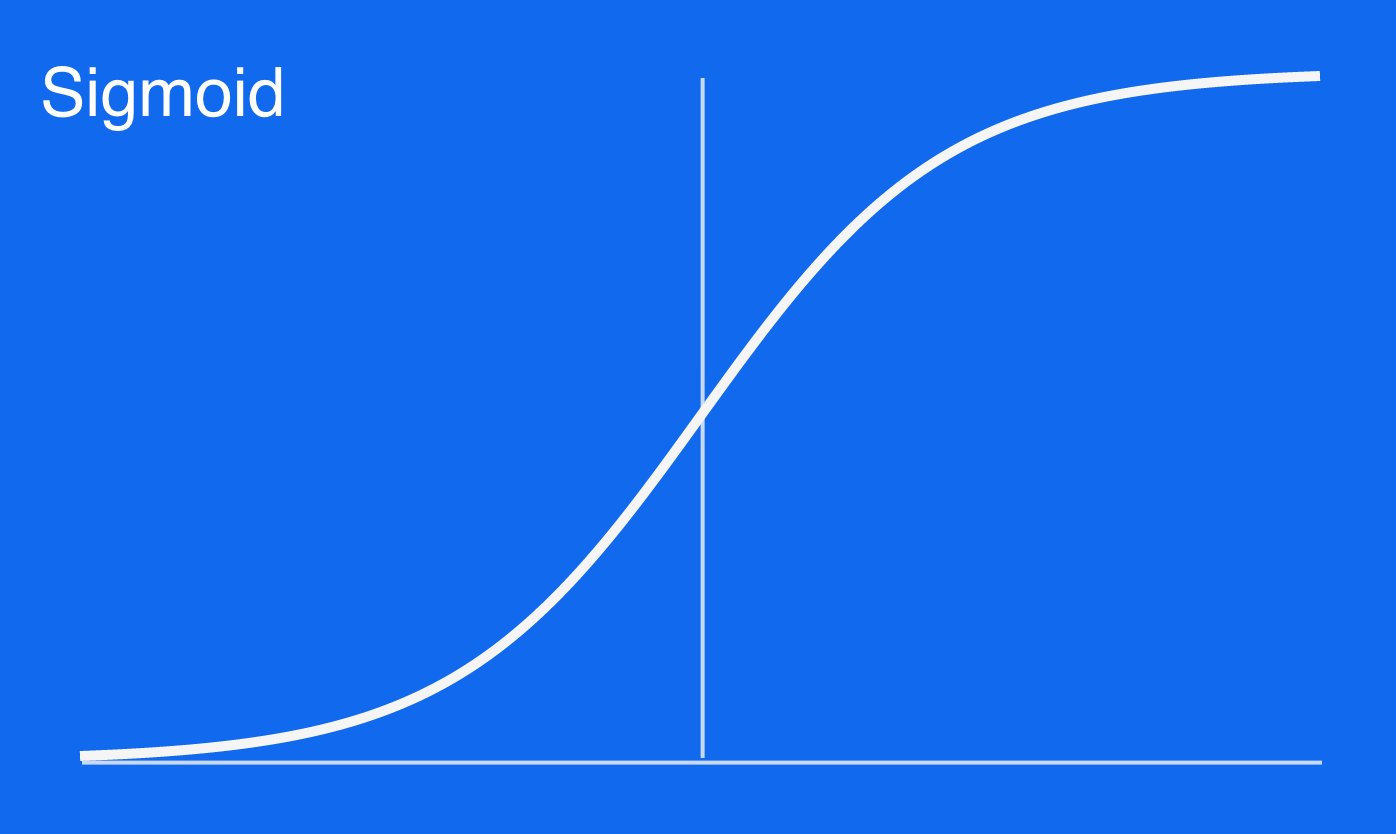
\includegraphics[width=.265\textwidth]{fig/sigmoid.png}
\caption{Sigmoid activation function.}
\end{figure}


\paragraph{Hyperbolic Tangent}.\\\\
Much like the sigmoid function in both advantages and disadvantages. The hyperbolic tangent function provides a smooth curve which is zero centred. It is however computationally expensive and suffers from the vanishing gradient problem.  

\begin{equation}
    f(x) = \frac {e^x - e^{-x}} {e^x + e^{-x}}
\end{equation}
\begin{figure}[H]
\centering
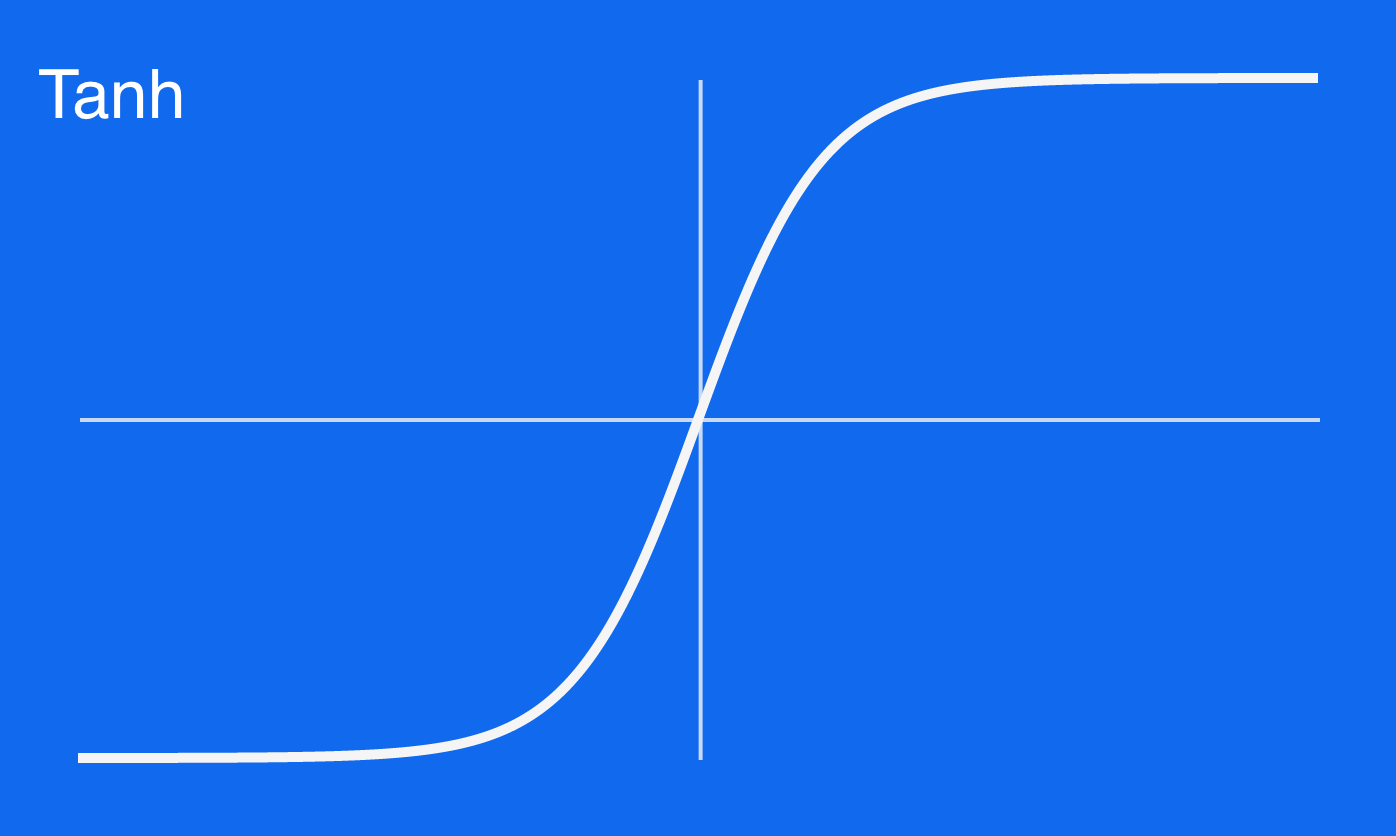
\includegraphics[width=.265\textwidth]{fig/tanh.png}
\caption{Tanh activation function.}
\end{figure}


\paragraph{Rectified Linear Unit}.\\\\
A commonly used activation for large deep neural networks, due to its computational efficiency and quick convergence. It is non-linear although it appears like a linear function, and allows for back propagation. It does however suffer from the dying ReLU problem - when inputs tend to zero or below, the gradient of the function becomes zero and the network cannot perform backpropagation to learn. 

\begin{equation}
f(x) = 
    \begin{cases}
      0 , & \mathbf{if} \ x < threshold \\
      x , & \text{otherwise}\\
    \end{cases}
  \end{equation}
\begin{figure}[H]
\centering
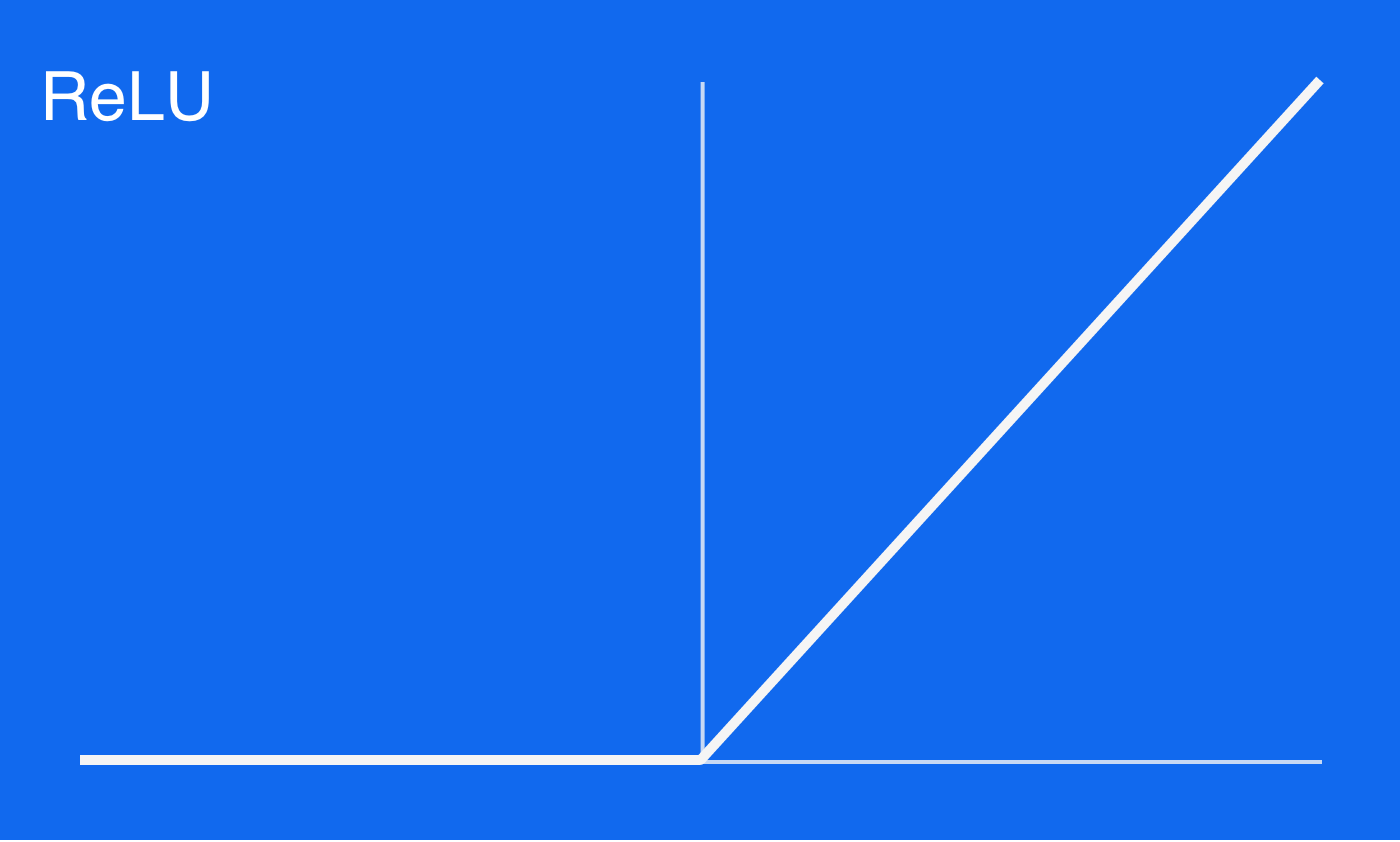
\includegraphics[width=.265\textwidth]{fig/relu.png}
\caption{ReLU activation function.}
\end{figure}



\paragraph{Swish}.\\\\
https://arxiv.org/abs/1710.05941v1
\textbf{\textit{a new, self-gated activation function discovered by researchers at Google. According to their paper, it performs better than ReLU with a similar level of computational efficiency. In experiments on ImageNet with identical models running ReLU and Swish, the new function achieved top -1 classification accuracy 0.6-0.9\% higher.}}

\begin{equation}
f(x) = x/1-e^{-x}
  \end{equation}
\begin{figure}[H]
\centering
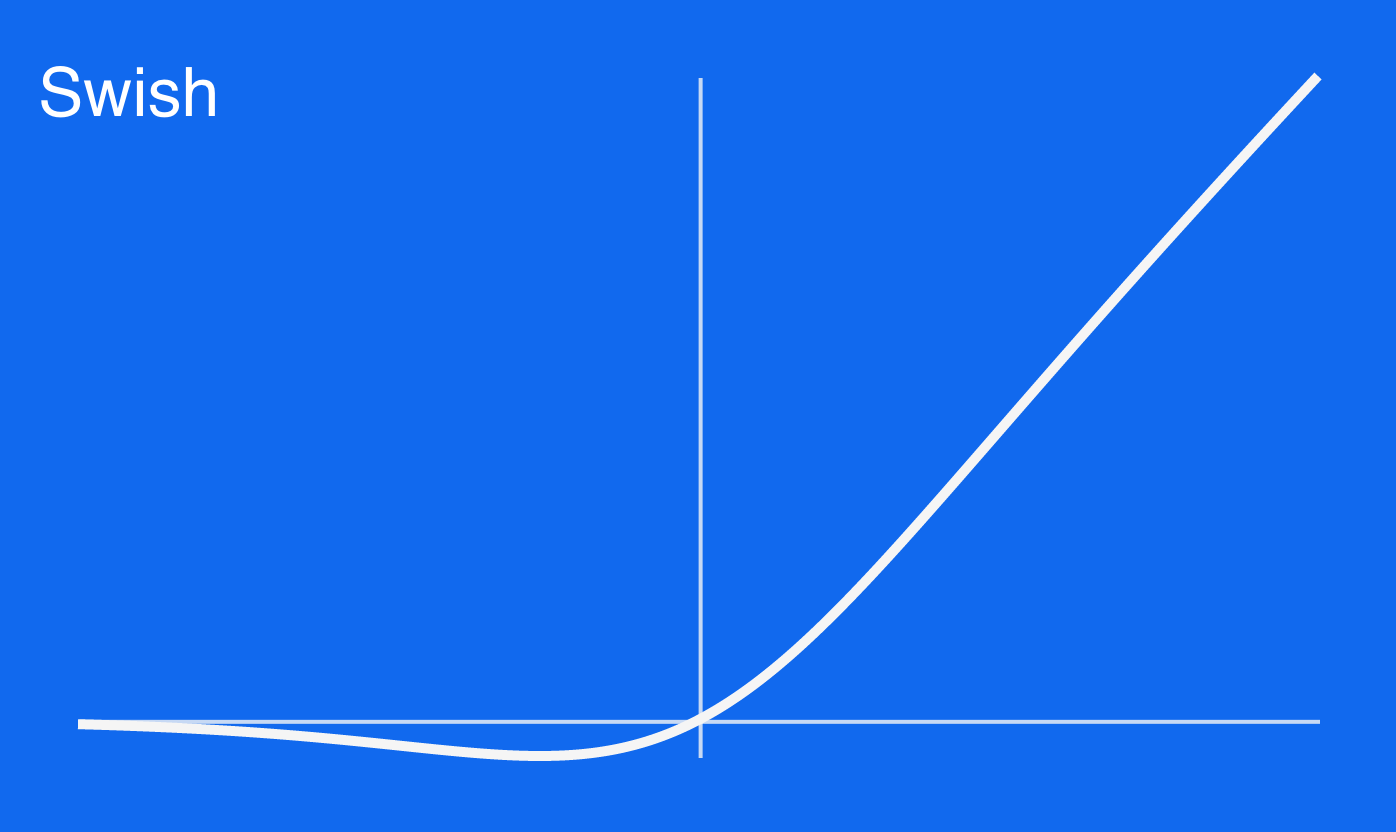
\includegraphics[width=.265\textwidth]{fig/swish.png}
\caption{Swish activation function.}
\end{figure}

\paragraph{\textbf{A note on backpropagation}}
\emph{As it has not been explicitly explained before back-propagation is an algorithm used to train neural networks. The derivative (or gradient) of an activation function is important in the use of back propagation. Here the model weights are adjusted, and improved, by tracing back all the connections in network, suggesting an optimal weight of each neuron.} 

\subsubsection{Demonstration of non-linear activation functions}

To demonstrate the effect of these we take a sample isopleth of Methane and Ozone, reduce it to two dimensions, and then reconstruct it. Here we can see that some of the non-linearity of the original dataset has been lost when discarding the third principle component during PCA. Using a tanh activation function in an auto-encoder however recreates much of the original properties of the data. 


\begin{figure}[H]

\begin{subfigure}{.33\textwidth}
  \centering
  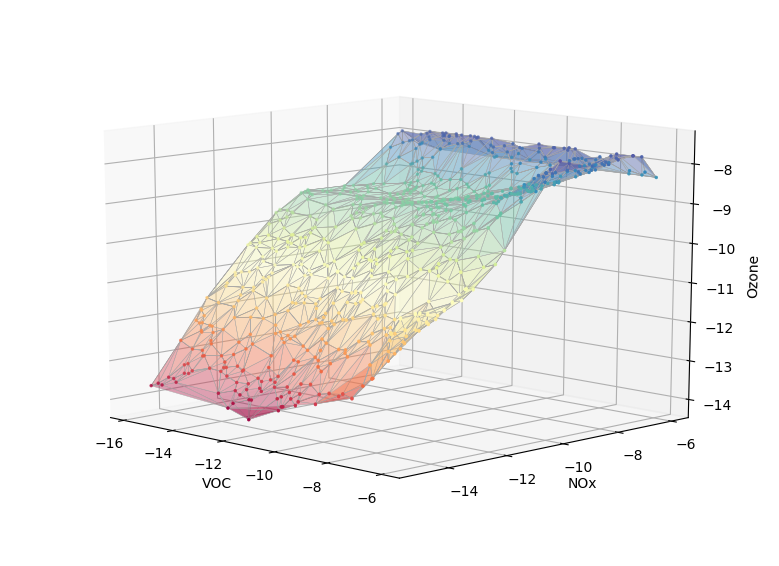
\includegraphics[width=\textwidth]{fig/original.png}
  \label{fig:orig}
  \caption{Original}
\end{subfigure}%
\begin{subfigure}{.33\textwidth}
  \centering
  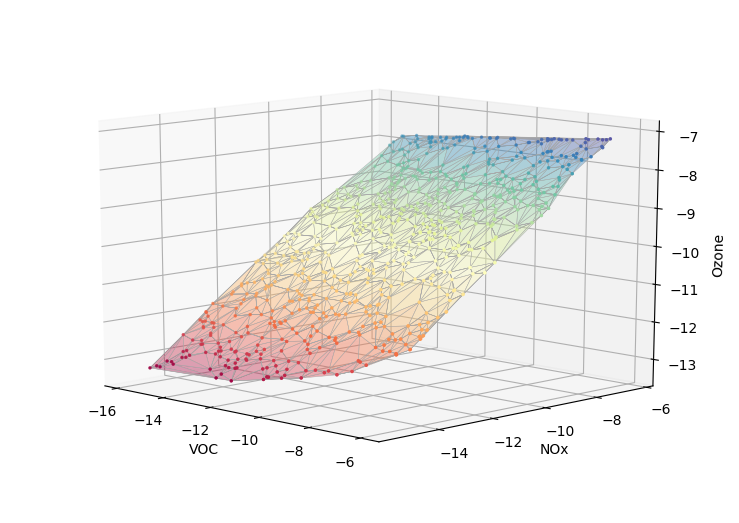
\includegraphics[width=\textwidth]{fig/rpca.png}
  \label{fig:pca}
  \caption{PCA}
\end{subfigure}%
\begin{subfigure}{.33\textwidth}
  \centering
  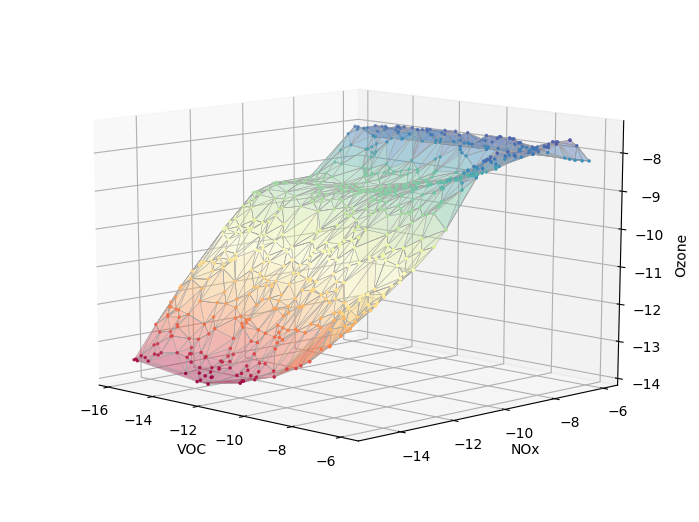
\includegraphics[width=\textwidth]{fig/rae.png}
  \label{fig:ae}
  \caption{AE (Tanh)}
\end{subfigure}%


\caption{Reducing the original dataset by 1 dimension and reconstructing it using different methods. Figure created using 300 simulations initialised with NOx (variable), Methane (variable) and Ozone (constant) using a latin hypercube. The results are then plotted and converted into a surface using delaunay triangulation. }
\end{figure}


\subsection{Graph Auto-Encoders (GAE)}

It was seen that graphs neural networks (GNN) were far more powerful in 2016....
Training time and results\\

Graph auto-encoders are an extension to these, applying the auto-encoder structure to a GNN.Here we may feed information about the relationships between items in our network, as well as the features representing them. 

This method of representation has its purpose in both classification and link prediction. In terms of an autoencoder, we may use this to extract the graph embeddings at a lower dimension. In \cite{karatAE} it is shown that GAEs are able to extract an embedding of the graph communities within a network. In other papers, GAEs have been used for matrix completion, and in-turn link prediction \cite{gaelink}. This makes them a potentially powerful tool in the visualisation, understanding and prediction of atmospheric chemical graphs. 

 





\section{Results: Part I}

In order to get a representation of the mechanism we run 300 randomly initiated scenarios, with the experimental design capable of accepting more data at a later point. We then extract the lifetimes from the diagonal of the jacobian, and convert them into vectors representing the duration of all 3 days for each simulation. These vectors are then compared against eachother to find species of similar lifetimes, which follow a like response to the diurnal cycle. This is done through the use of euclidian and cosine similarities. 

\subsection{Temporal Lifetime Vector Comparison}
First we wish to explore the results of a single simulation. This will help establish the thresholds and methodology that is to be used in future examples. As we do not wish to lump inorganics, we remove these from the program and generate all the pairwise interactions between species. We compute the euclidean and cosine distances for all remaining reaction pairs (88410 pairs) across the entirety of the single calculation. These are then plotted on separate axis, and coloured using the geometric mean, \autoref{fig:metric}. \\

Since there are $n^2$ different combinations, this process can be lengthy to compute. Moreover the number of nodes present makes it difficult to visually determine which couplets to lump together, especially when they are overlaying eachother, as in \autoref{fig:morig}. To overcome this we apply a force graph simulation to each node. Here a strong force pulls them towards their true location, whist a collision/repulsive force ensures that there exists no overlap between nodes. Although some information loss may be incurred this way, it does enable us to interactively determine which pairs belong to which points.   

Plotting the data this way provides an approximate view of how lifetimes change within the system. \autoref{fig:density} shows the distribution of values across both metrics. Here we see that although there is some difference the cosine difference can be used as an indicator for exploring further. This is useful since the cosine difference is a matrix operation and can produce near instant results in the form of the output relationship matrix. The euclidean distance however must be computed for each coupling individually as it requires taking the difference between the temporal lifetime arrays of each species. This means that rather than computing the euclidean distance for all permutaions of species, we can compute only those whose cosine distances suggest potentially promising results.  



\begin{figure}[H]
\begin{subfigure}{.5\textwidth}
  \centering
  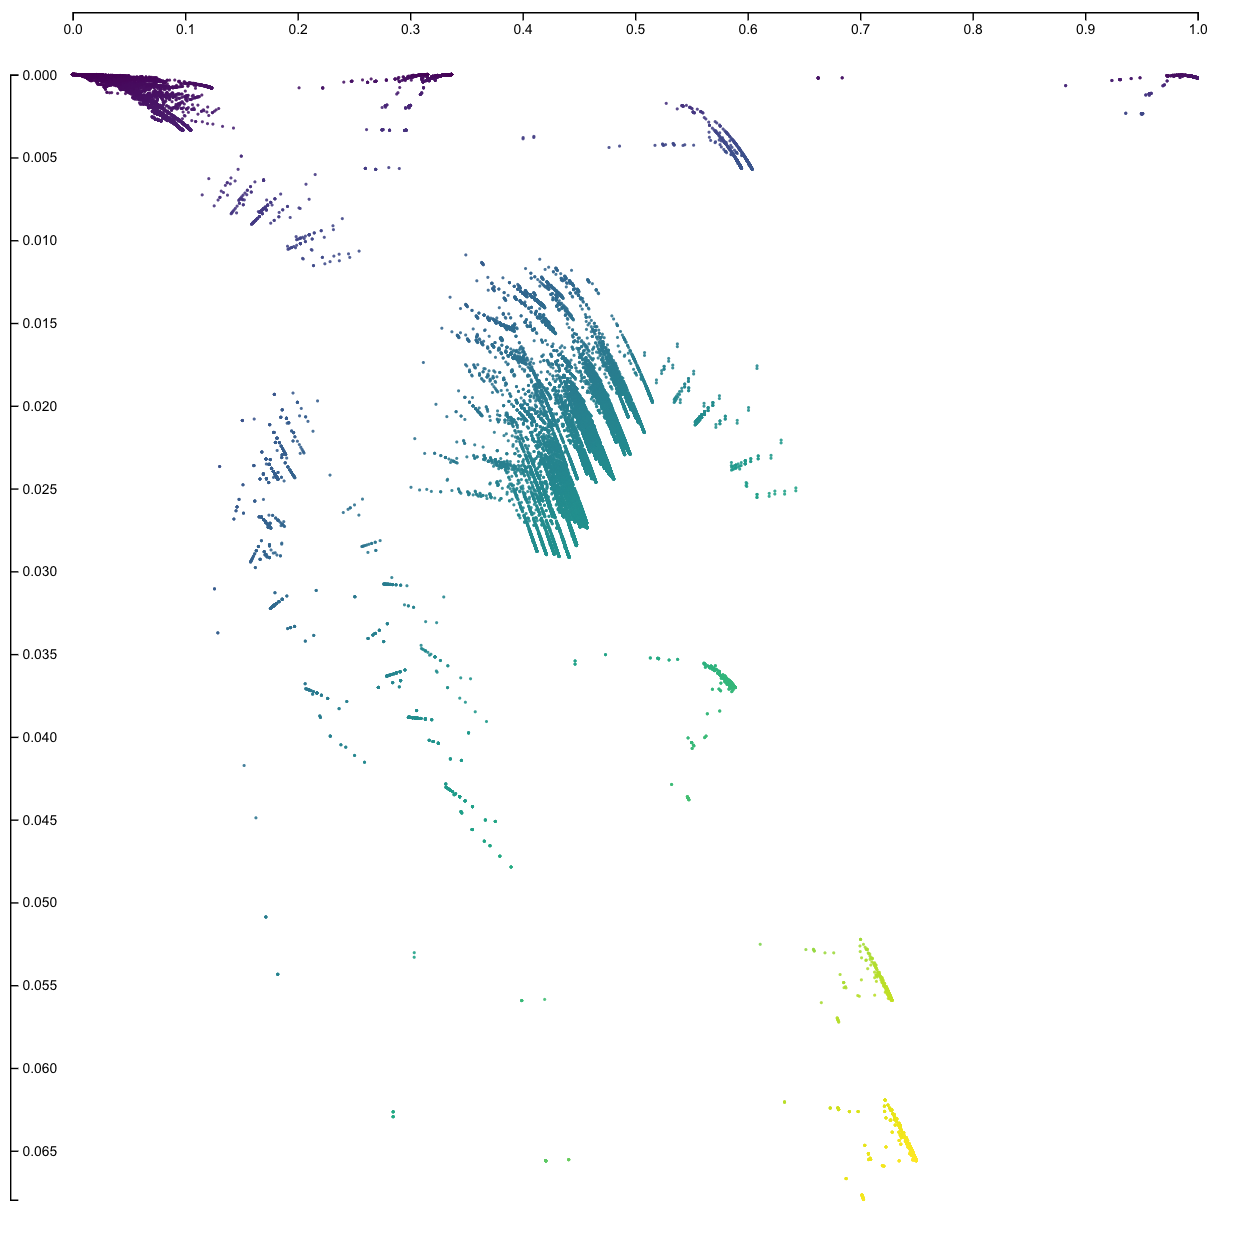
\includegraphics[width=\textwidth]{fig/metric-1.png}
  \label{fig:morig}
  \caption{Original}
\end{subfigure}%
\begin{subfigure}{.5\textwidth}
  \centering
  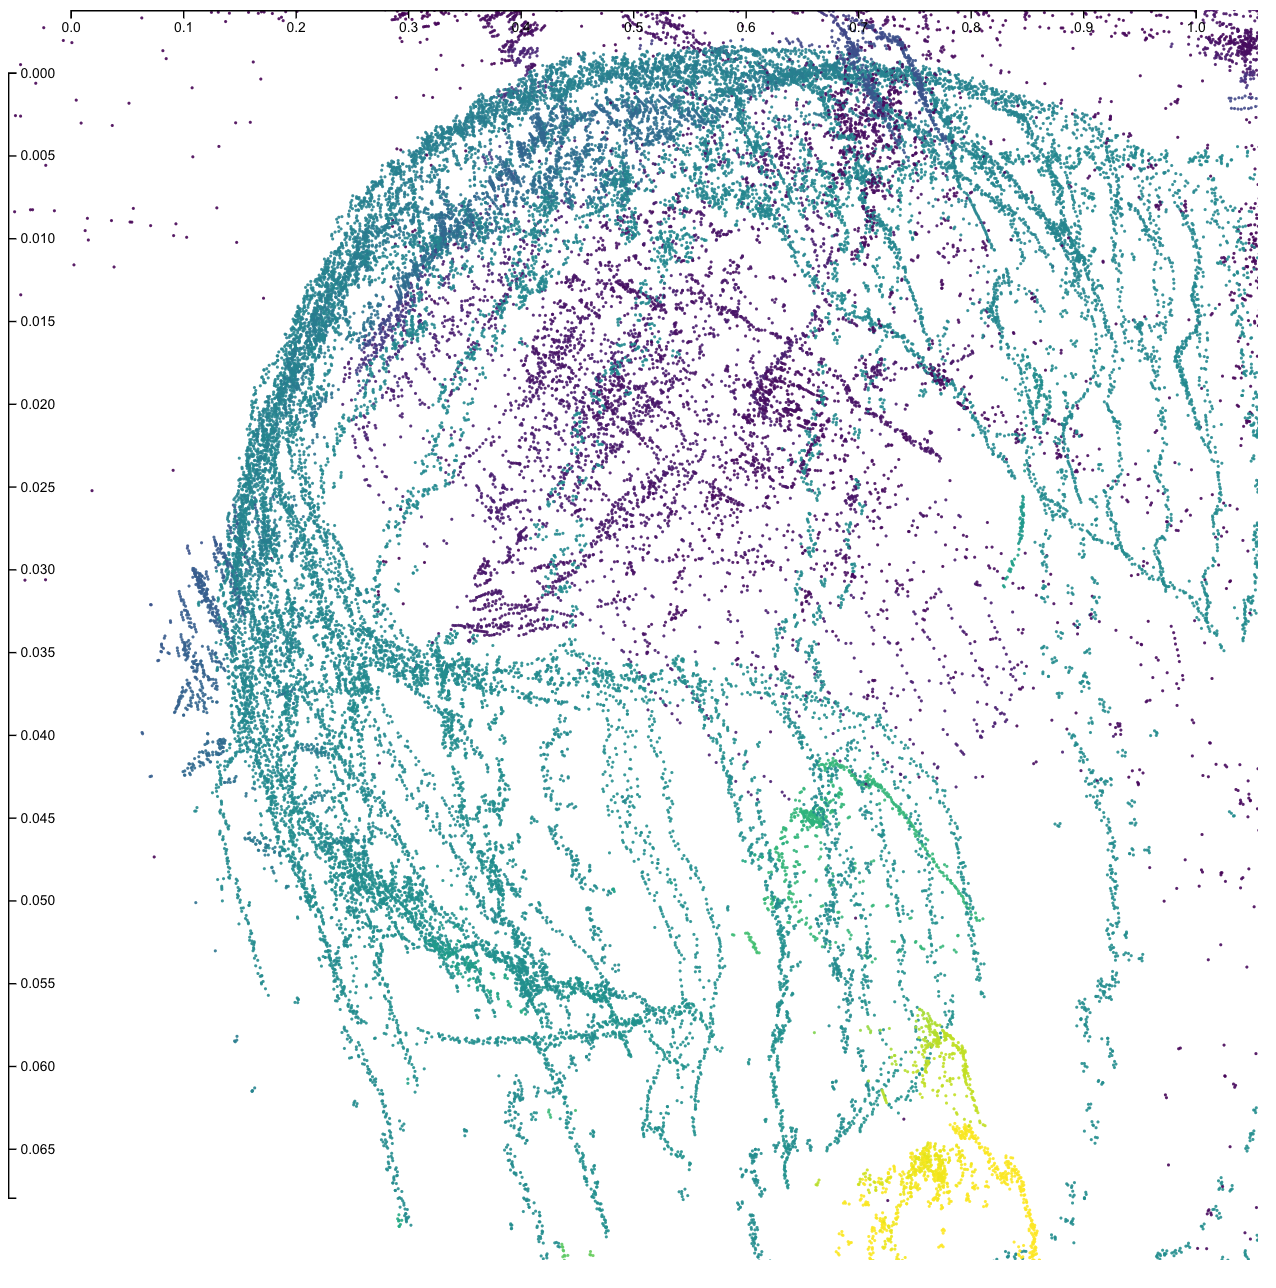
\includegraphics[width=\textwidth]{fig/metric0.png}
  \label{fig:m1}
  \caption{First collision detection timestep, before attractive forces have fully kicked in.}
\end{subfigure}

\caption{Showing the evolution from the original overlaid locations, \autoref{fig:morig} to the slightly more accessible (interactively) \autoref{fig:metric}}
\end{figure}


\begin{figure}

\begin{subfigure}{.5\textwidth}
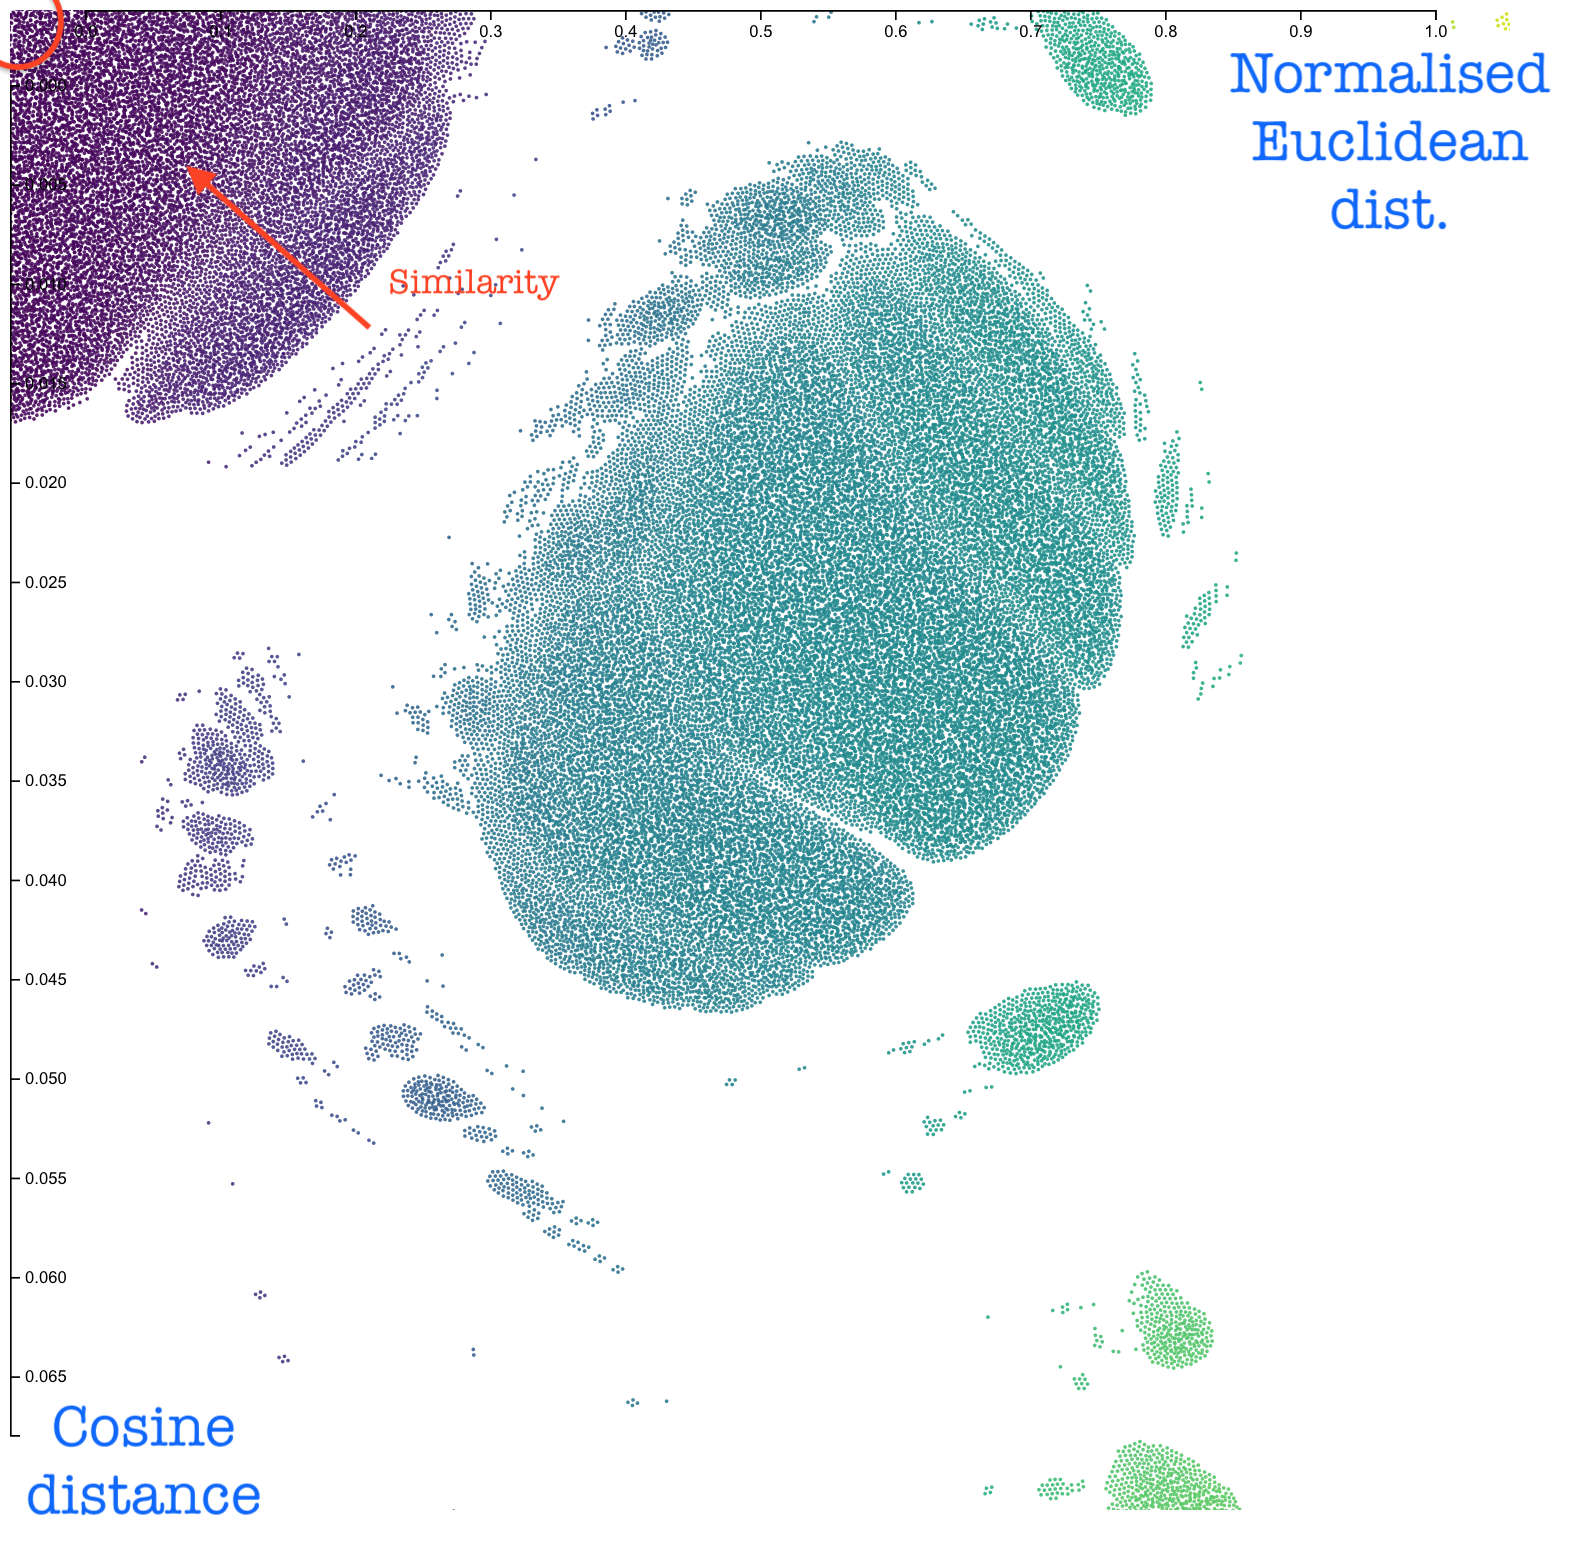
\includegraphics[width=\textwidth]{fig/metric.png}
\label{fig:metric}
\caption{Interactive, non overlapping plot of normalised euclidian distance across the x axis against the cosine distance on the y. The colouring is the geometric mean between them.}
\end{subfigure}
\begin{subfigure}{.5\textwidth}
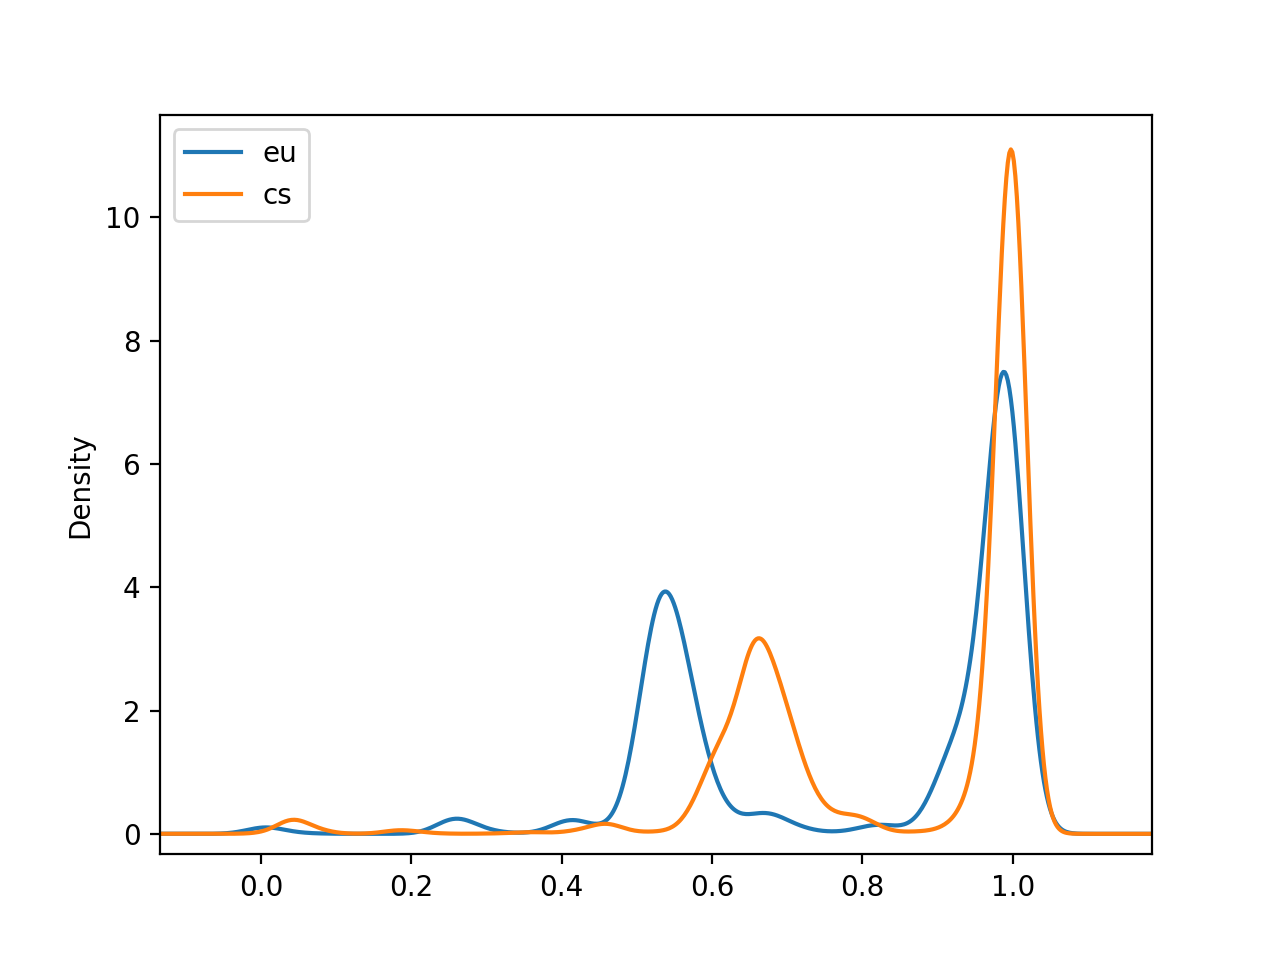
\includegraphics[width=\textwidth]{fig/metric_density.png}
\label{fig:density}
\caption{Gaussian Kernel Density Estimate plot showing the distributions present for each distance metric}
\end{subfigure}
\caption{Showing the evolution from the original overlaid locations, \autoref{fig:morig} to the slightly more accessible (interactively) \autoref{fig:metric}}
\end{figure}


\subsection{Viewing the similarity graph}

One method to simplify this is to convert to the pairwise interaction list into a fully connected graph. Here we have individual species, pulled together by the similarity (geometric mean) between each two nodes.
Unfortunately in being a complete graph of  421 species and 88410 links, this is quite difficult to visualise without forming a \emph{hairball} [fig a]. As a means of filtering the results we trim the weakest links in sequence. This produces rings of densely connected species based on lifetime thresholds which corresponds to the different types of chemsitry species undergo \\



\textbf{Need to find out what the abbreviated names in cri stand for!}. The sizes and species within each ring show similararities to the distance metric plot as would be expected. This provides an alternative representation where graph community detection algorithms such as MCL [ref] can be used to isolate chemistry with different levels of lifetime relationships between them. Unfortunately, as we are interested species with near identical lifetimes, this does not hold a great deal of merit in locating these. 


\begin{figure}[H]

\begin{subfigure}{.33\textwidth}
  \centering
  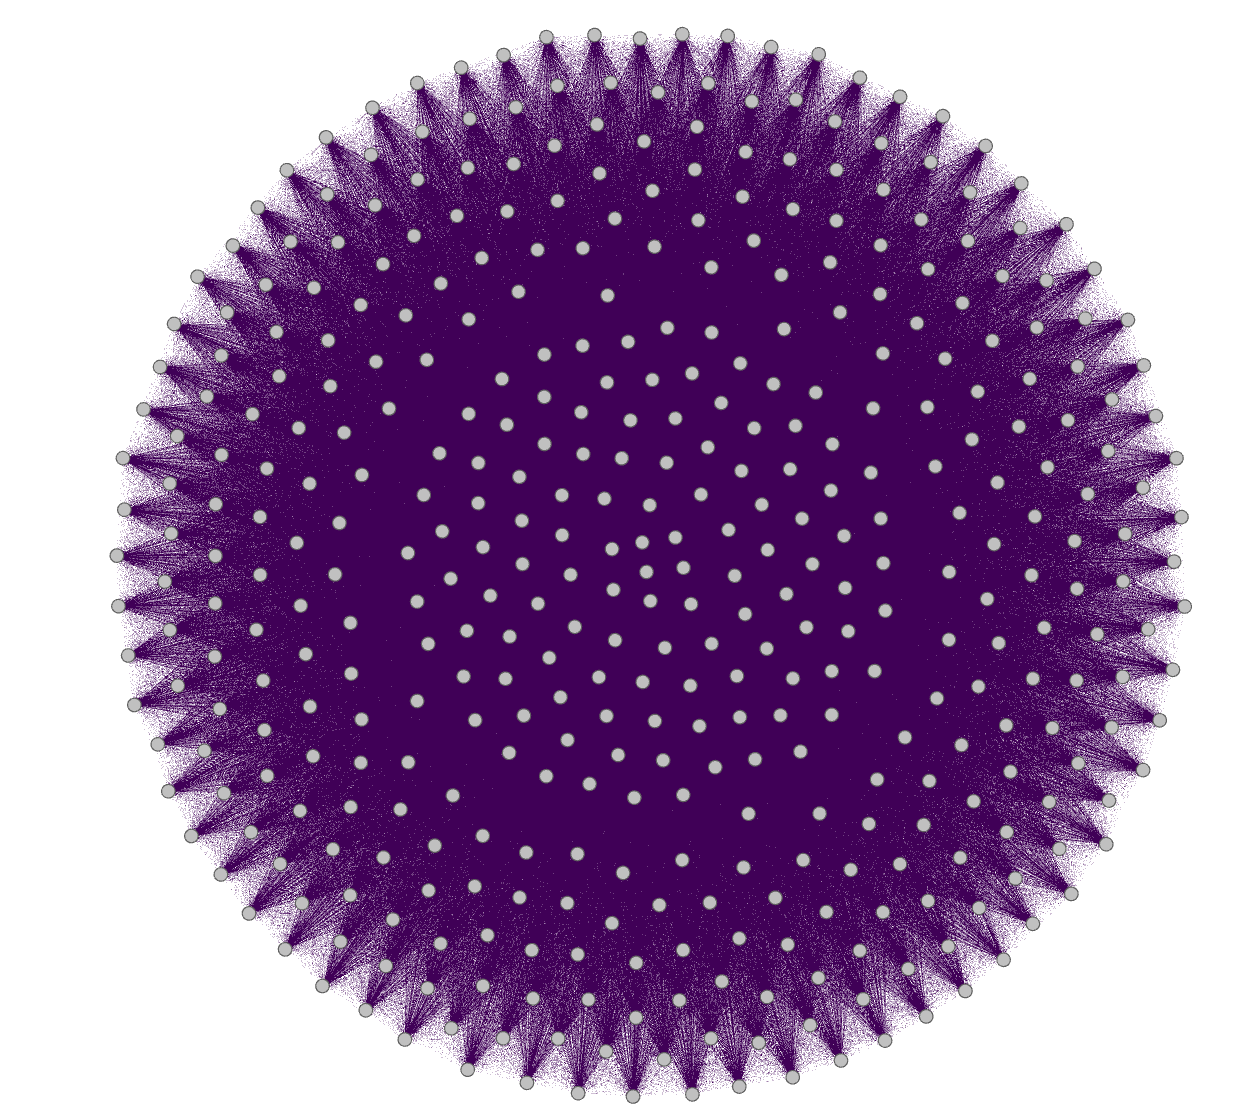
\includegraphics[width=\textwidth]{fig/step1.png}
  \label{fig:orig}
  \caption{Initial connected graph}
\end{subfigure}%
\begin{subfigure}{.33\textwidth}
  \centering
  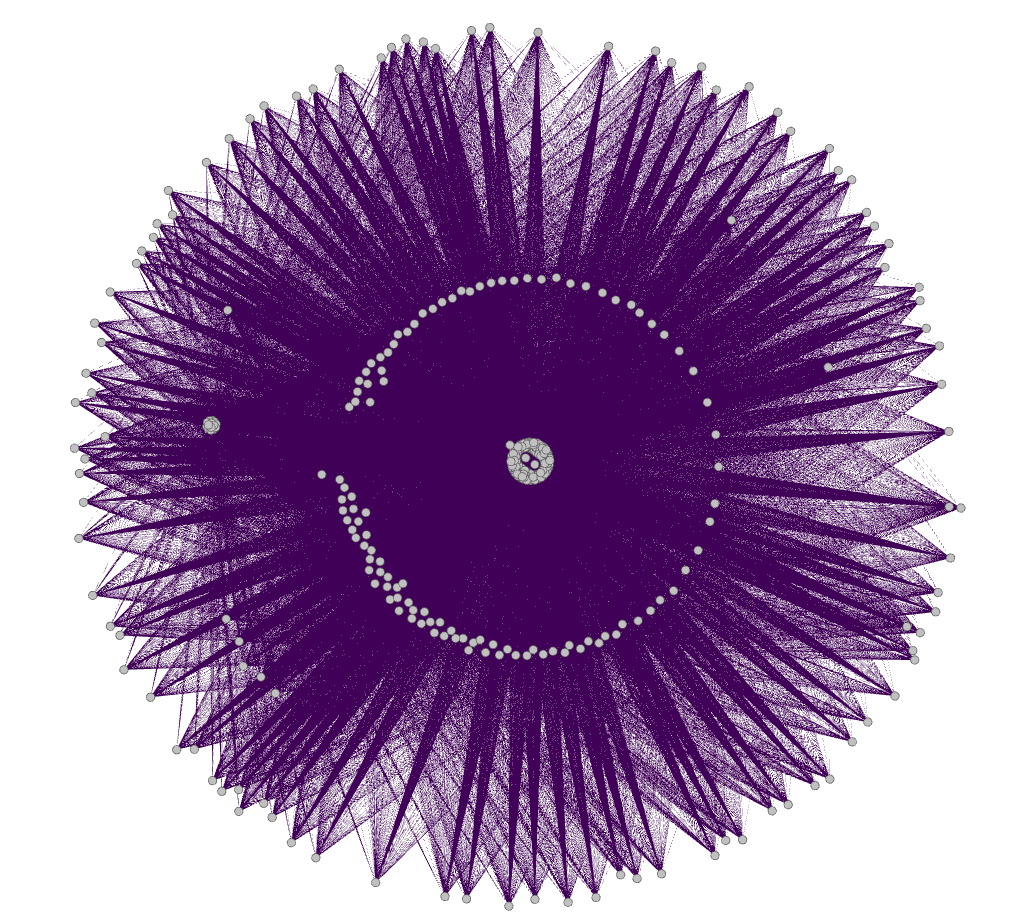
\includegraphics[width=\textwidth]{fig/step2.png}
  \label{fig:pca}
  \caption{Initial graph with trimming ~ half the edges}
\end{subfigure}%
\begin{subfigure}{.33\textwidth}
  \centering
  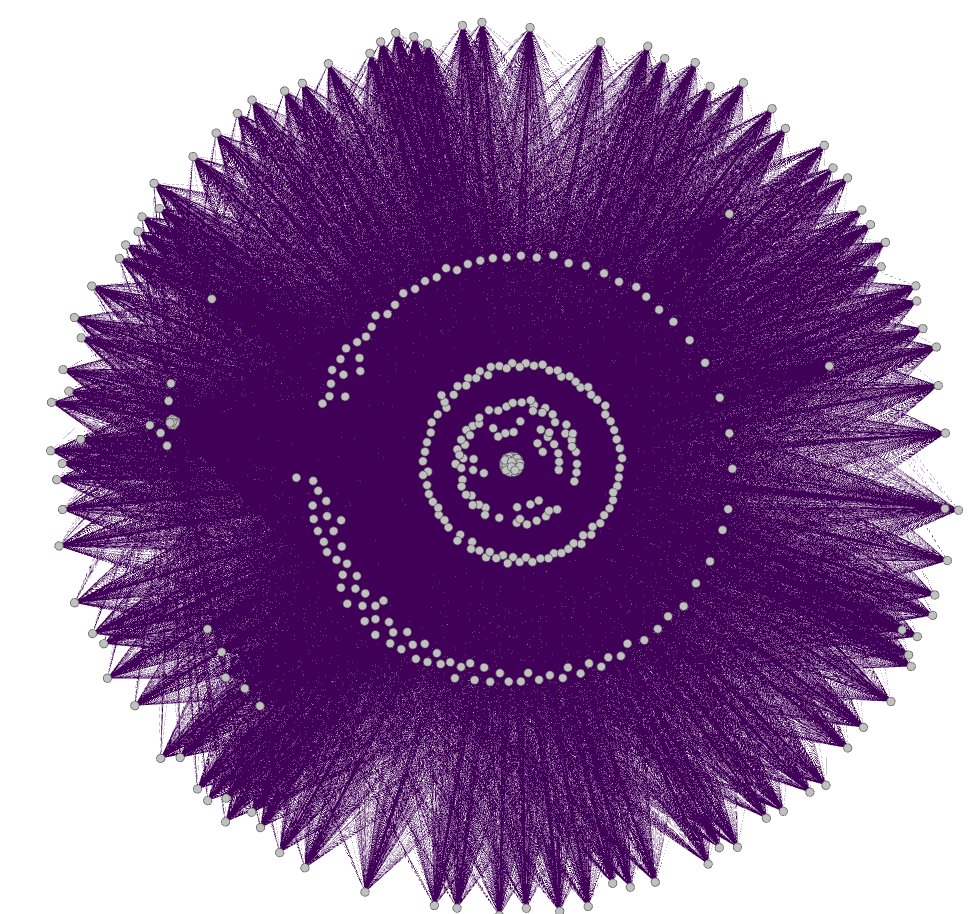
\includegraphics[width=\textwidth]{fig/step3.png}
  \label{fig:ae}
  \caption{Heavy trimming.}
\end{subfigure}%


\caption{A froce graph with progressive trimming of weak, poorly related, edges.}
\end{figure}

\subsubsection{Using MCMC to extract groups}

Need to see what Cri names mean to better explain these. 


\subsection{Comparing to the graph encodings}

Next we can make use of the dimensionality reduction properties of the graph autoencoder. Here we can supply the mechanistic network structure to the algorithm, as well as the geometric means, cosine and euclidian distances as features of each node (TBC Plot 1). We can then compare this to the embedding created by using the complete relationship graph as above, and the lifetimes of each species as their features. In comparing these two plots, we can check the ability of the gae to extract information of interest. 


\begin{figure}[H]
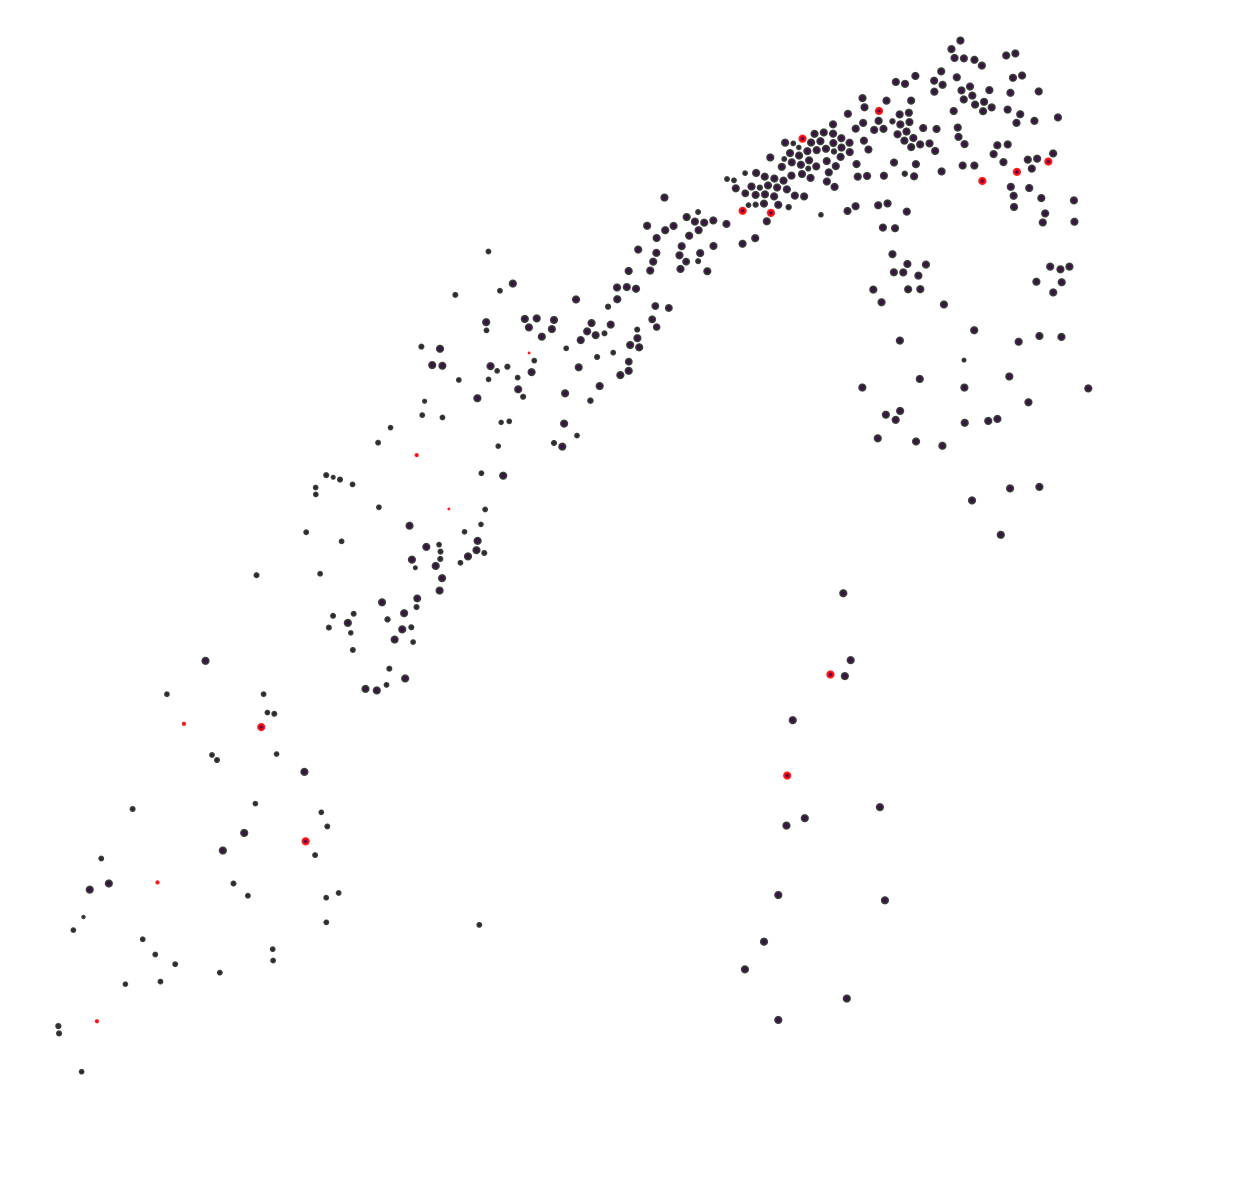
\includegraphics[width=.5\textwidth]{fig/aedist.png}
\caption{Testing trying to supply the cosine relationship matrix as a graph, and the euclidian distance matrix as node features. Only 1 training cycle.}
\end{figure}

\begin{table}
\centering
\begin{tabular}{lr}
\toprule
Pairings &  Geometric Mean \\
\midrule
CH3CO3\_CARB9      &        0.000000 \\
HOCH2CO3\_CARB9    &        0.000000 \\
C2H5CO3\_CARB9     &        0.000000 \\
DHPR12O2\_CH3OCHO  &        0.000000 \\
MACO3\_CARB9       &        0.000189 \\
CO\_DHPR12O2       &        0.002915 \\
DHPR12O2\_C2H6     &        0.003488 \\
DHPR12O2\_DMC      &        0.005956 \\
DHPR12O2\_METHACET &        0.006638 \\
RU10AO2\_CH3OCHO   &        0.008171 \\
CH3COCH3\_DHPR12O2 &        0.008589 \\
DHPR12O2\_HCOOH    &        0.008589 \\
CO\_RU10AO2        &        0.008666 \\
RU10AO2\_C2H6      &        0.008875 \\
DHPR12O2\_TBUACET  &        0.009399 \\
DHPR12O2\_CH3NO3   &        0.009437 \\
RU10AO2\_DMC       &        0.010112 \\
CH3CO3\_CARB12     &        0.010267 \\
C2H5CO3\_CARB12    &        0.010267 \\
HOCH2CO3\_CARB12   &        0.010267 \\
\bottomrule
\end{tabular}\caption{The 20 most `similar' species lifetimes provided by taking the geometric mean of the euclidean and cosine distances.}
\end{table}


\section{Methodology: Part II}

\subsection{Infomap Clustering}


Insert infomap chapter here
\section{Results II}


\section{Methodology: Part II - Comparing both styles}

\section{Results III}


\section{Conclusion}

\tableofcontents

\bibliographystyle{pasa-mnras}
\bibliography{bibliography}

\end{document}
